\documentclass[12pt,letterpaper,reqno]{article}

% \usepackage{mathtools}
\usepackage{epsfig}
\usepackage{amsmath}
\usepackage{amssymb}
\usepackage{amsthm}
\usepackage{indentfirst}
\usepackage{xspace}
\usepackage{multirow}
\usepackage{hyperref}
\usepackage{xcolor}
\usepackage{verbatim}
\usepackage[letterpaper,margin=1in,headheight=15pt]{geometry}
\usepackage{mathpazo}
\usepackage{tikz-cd}
\usepackage{booktabs}
\usepackage{framed}
\usepackage{float}
\usepackage{thmtools}
\usepackage{dashrule}
\usepackage[missing=]{gitinfo2}
\usepackage{fancyhdr}
\usepackage{enumerate}
\usepackage{graphicx}
\usepackage{mathrsfs}
\usepackage{calligra}
\usepackage[titletoc,title]{appendix}

\definecolor{darkblue}{rgb}{0.1,0.1,0.7}
\definecolor{darkred}{rgb}{0.5,0.1,0.1}
\definecolor{darkgreen}{rgb}{0.0,0.42,0.06}
\hypersetup{colorlinks=true,urlcolor=darkred,linkcolor=darkblue,citecolor=darkred}
\definecolor{shadecolor}{rgb}{0.85,0.85,0.85}

% Bibliography formatting
\usepackage[bibstyle=authoryear-comp,labeldate=false,defernumbers=true,maxnames=20,uniquename=init,dashed=false,backend=biber,sorting=none]{biblatex}

\DeclareNameAlias{sortname}{first-last}

\DeclareFieldFormat{url}{\url{#1}}
\DeclareFieldFormat[article]{pages}{#1}
\DeclareFieldFormat[inproceedings]{pages}{\lowercase{pp.}#1}
\DeclareFieldFormat[incollection]{pages}{\lowercase{pp.}#1}
\DeclareFieldFormat[article]{volume}{\textbf{#1}}
\DeclareFieldFormat[article]{number}{(#1)}
\DeclareFieldFormat[article]{title}{\MakeCapital{#1}}
\DeclareFieldFormat[inproceedings]{title}{#1}
\DeclareFieldFormat{shorthandwidth}{#1}

% Don't use "In:" in bibliography. Omit urls from journal articles.
\DeclareBibliographyDriver{article}{%
  \usebibmacro{bibindex}%
  \usebibmacro{begentry}%
  \usebibmacro{author/editor}%
  \setunit{\labelnamepunct}\newblock
  \MakeSentenceCase{\usebibmacro{title}}%
  \newunit
  \printlist{language}%
  \newunit\newblock
  \usebibmacro{byauthor}%
  \newunit\newblock
  \usebibmacro{byeditor+others}%
  \newunit\newblock
  \printfield{version}%
  \newunit\newblock
%  \usebibmacro{in:}%
  \usebibmacro{journal+issuetitle}%
  \newunit\newblock
  \printfield{note}%
  \setunit{\bibpagespunct}%
  \printfield{pages}
  \newunit\newblock
  \usebibmacro{eprint}
  \newunit\newblock
  \printfield{addendum}%
  \newunit\newblock
  \usebibmacro{pageref}%
  \usebibmacro{finentry}}

% Remove dot between volume and number in journal articles.
\renewbibmacro*{journal+issuetitle}{%
  \usebibmacro{journal}%
  \setunit*{\addspace}%
  \iffieldundef{series}
    {}
    {\newunit
     \printfield{series}%
     \setunit{\addspace}}%
  \printfield{volume}%
%  \setunit*{\adddot}%
  \printfield{number}%
  \setunit{\addcomma\space}%
  \printfield{eid}%
  \setunit{\addspace}%
  \usebibmacro{issue+date}%
  \newunit\newblock
  \usebibmacro{issue}%
  \newunit}


% Bibliography categories
\def\makebibcategory#1#2{\DeclareBibliographyCategory{#1}\defbibheading{#1}{\section*{#2}}}
\makebibcategory{books}{Books}
\makebibcategory{papers}{Refereed research papers}
\makebibcategory{chapters}{Book chapters}
\makebibcategory{conferences}{Papers in conference proceedings}
\makebibcategory{techreports}{Unpublished working papers}
\makebibcategory{bookreviews}{Book reviews}
\makebibcategory{editorials}{Editorials}
\makebibcategory{phd}{PhD thesis}
\makebibcategory{subpapers}{Submitted papers}
\makebibcategory{curpapers}{Current projects}

\setlength{\bibitemsep}{2.65pt}
\setlength{\bibhang}{.8cm}
\renewcommand{\bibfont}{\small}

\renewcommand*{\bibitem}{\addtocounter{papers}{1}\item \mbox{}\hskip-0.85cm\hbox to 0.85cm{\hfill\arabic{papers}.~~}}
\defbibenvironment{bibliography}
{\list{}
  {\setlength{\leftmargin}{\bibhang}%
   \setlength{\itemsep}{\bibitemsep}%
   \setlength{\parsep}{\bibparsep}}}
{\endlist}
{\bibitem}

\newenvironment{publications}{\section{\LARGE Publications}\label{papersstart}\vspace*{0.2cm}\small
\titlespacing{\section}{0pt}{1.5ex}{1ex}\itemsep=0.00cm
}{\label{papersend}\addtocounter{sumpapers}{-1}\refstepcounter{sumpapers}\label{sumpapers}}

\def\printbib#1{\printbibliography[category=#1,heading=#1]\lastref{sumpapers}}

% Counters for keeping track of papers
\newcounter{papers}\setcounter{papers}{0}
\newcounter{sumpapers}\setcounter{sumpapers}{0}
\def\lastref#1{\addtocounter{#1}{\value{papers}}\setcounter{papers}{0}}

% theorem environments
\declaretheoremstyle[spaceabove=0.25cm,spacebelow=0.25cm,notefont=\normalfont\bfseries, notebraces={(}{)}]{theorem}
\declaretheoremstyle[spaceabove=0.25cm,spacebelow=0.25cm,bodyfont=\normalfont,notefont=\normalfont\bfseries, notebraces={(}{)}]{noital}
\declaretheoremstyle[spaceabove=0.25cm,spacebelow=0.25cm,bodyfont=\normalfont\color{darkgreen},notefont=\normalfont\bfseries, notebraces={(}{)}]{green}
\declaretheoremstyle[spaceabove=0.25cm,spacebelow=0.25cm,bodyfont=\normalfont,notefont=\normalfont\bfseries,qed=$\qedsymbol$,notebraces={(}{)}]{proofstyle}

\declaretheorem[name=Theorem,numberwithin=section,style=theorem]{thm}
\declaretheorem[name=Proposition,sibling=thm,style=theorem]{prop}
\declaretheorem[name=Corollary,sibling=thm,style=theorem]{cor}
\declaretheorem[name=Lemma,sibling=thm,style=theorem]{lem}
\declaretheorem[name=Definition,sibling=thm,style=noital]{defn}
\declaretheorem[name=Example,sibling=thm,style=noital]{example}
\declaretheorem[name=Exercise,numberwithin=section,style=green]{exercise}
\declaretheorem[name=Proof,style=proofstyle,numbered=no]{pf}

\numberwithin{equation}{section}


% macros for convenience
\newcommand{\tops}{\texorpdfstring}

\newcommand{\nid}{\noindent}

\newcommand{\fa}{{\mathfrak a}}
\newcommand{\fp}{{\mathfrak p}}
\newcommand{\fk}{{\mathfrak k}}
\newcommand{\fg}{{\mathfrak g}}
\newcommand{\fh}{{\mathfrak h}}
\newcommand{\fn}{{\mathfrak n}}
\newcommand{\fq}{{\mathfrak q}}
\newcommand{\fm}{{\mathfrak m}}
\newcommand{\fr}{{\mathfrak r}}
\newcommand{\fu}{{\mathfrak u}}
\newcommand{\fG}{{\mathfrak G}}

\newcommand{\cC}{\ensuremath{\mathcal C}}
\newcommand{\cG}{\ensuremath{\mathcal G}}
\newcommand{\cB}{\ensuremath{\mathcal B}}
\newcommand{\cL}{\ensuremath{\mathcal L}}
\newcommand{\cS}{\ensuremath{\mathcal S}}
\newcommand{\cF}{\ensuremath{\mathcal F}}
\newcommand{\cK}{\ensuremath{\mathcal K}}
\newcommand{\cZ}{\ensuremath{\mathcal Z}}
\newcommand{\cM}{\ensuremath{\mathcal M}}
\newcommand{\cN}{\ensuremath{\mathcal N}}
\newcommand{\cO}{\ensuremath{\mathcal O}}
\newcommand{\cH}{\ensuremath{\mathcal H}}
\newcommand{\cX}{\ensuremath{\mathcal X}}
\newcommand{\cY}{\ensuremath{\mathcal Y}}
\newcommand{\cA}{\ensuremath{\mathcal A}}
\newcommand{\cI}{\ensuremath{\mathcal I}}

\newcommand{\R}{\ensuremath{\mathbb R}}
\newcommand{\C}{\ensuremath{\mathbb C}}
\newcommand{\PP}{\ensuremath{\mathbb P}}
\newcommand{\Z}{\ensuremath{\mathbb Z}}
\newcommand{\Q}{\ensuremath{\mathbb Q}}
\newcommand{\A}{\ensuremath{\mathbb A}}
\newcommand{\bbH}{\ensuremath{\mathbb H}}
\newcommand{\bbI}{\ensuremath{\mathbb I}}
\newcommand{\bS}{\ensuremath{\mathbb S}}

\newcommand{\half}{\ensuremath{\frac{1}{2}}}
\newcommand{\qtr}{\ensuremath{\frac{1}{4}}}
\newcommand{\bq}{{\mathbf q}}
\newcommand{\N}{{\mathcal N}}
\newcommand{\F}{{\mathcal F}}
\newcommand{\HH}{{\mathcal H}}
\newcommand{\LL}{{\mathcal L}}
\newcommand{\RR}{{\mathcal R}}
\newcommand{\V}{{\mathcal V}}
\newcommand{\dirac}{\!\!\not\!\partial}
\newcommand{\Dirac}{\!\!\not\!\!D}
\newcommand{\cE}{{\mathcal E}}
\newcommand{\vs}{\not\!v}
\newcommand{\kahler}{K\"ahler\xspace}
\newcommand{\kq}{/\!\!/}
\newcommand{\kql}[1]{/\!\!/\!\!_#1\,}
\newcommand{\hk}{hyperk\"ahler\xspace}
\newcommand{\Hk}{Hyperk\"ahler\xspace}
\newcommand{\hkq}{/\!\!/\!\!/\!\!/}
\newcommand{\hkql}[1]{/\!\!/\!\!/\!\!/\!\!_#1\,}
\newcommand{\del}{\ensuremath{\partial}}
\newcommand{\delbar}{\ensuremath{\overline{\partial}}}
\newcommand{\I}{{\mathrm i}}
\newcommand{\J}{{\mathrm j}}
\newcommand{\K}{{\mathrm k}}
\newcommand{\e}{{\mathrm e}}
\newcommand\bid{{\mathbf 1}}
\newcommand{\de}{\mathrm{d}}
\newcommand{\ab}{\mathrm{ab}}
\newcommand{\vol}{\mathrm{vol}}
\renewcommand{\sf}{\mathrm{sf}}
\newcommand{\inst}{\mathrm{inst}}
\newcommand{\eff}{\mathrm{eff}}
\newcommand{\dR}{\mathrm{dR}}
\newcommand{\closed}{\mathrm{closed}}
\newcommand{\exact}{\mathrm{exact}}

\newcommand{\abs}[1]{\lvert#1\rvert}
\newcommand{\norm}[1]{\lVert#1\rVert}
\newcommand{\IP}[1]{\langle#1\rangle}
\newcommand{\DIP}[1]{\langle\!\langle#1\rangle\!\rangle}
\newcommand{\dwrt}[1]{\frac{\partial}{\partial#1}}
\newcommand{\eps}{\epsilon}
\newcommand{\simarrow}{\xrightarrow\sim}

\newcommand{\mmaref}[1]{}

\newcommand{\ti}[1]{\textit{#1}}
\newcommand{\tb}[1]{\textbf{#1}}
\newcommand{\lo}{\text{\calligra o}\,}
\newcommand{\dd}{\ensuremath{\mathscr{D}}}



\DeclareMathOperator{\ad}{ad}
\DeclareMathOperator{\im}{Im}
\DeclareMathOperator{\re}{Re}
\DeclareMathOperator{\Tr}{Tr}
\DeclareMathOperator{\End}{End}
\DeclareMathOperator{\Hom}{Hom}
\DeclareMathOperator{\Aut}{Aut}
\DeclareMathOperator{\Sym}{Sym}
\DeclareMathOperator{\Lie}{Lie}
\DeclareMathOperator{\diag}{diag}
\DeclareMathOperator{\Bun}{Bun}
\DeclareMathOperator{\Vect}{Vect}
\DeclareMathOperator{\Span}{Span}
\DeclareMathOperator{\grad}{grad}
\DeclareMathOperator{\rank}{rank}
\DeclareMathOperator{\ind}{ind}
\DeclareMathOperator{\coker}{coker}
\DeclareMathOperator{\Jac}{Jac}
\DeclareMathOperator{\Hol}{Hol}
\DeclareMathOperator{\gr}{gr}

\newcommand{\insfig}[2]{

\medskip
\noindent
\begin{minipage}{\linewidth}

\makebox[\linewidth]{\includegraphics[keepaspectratio=true,scale=#2]{figures/#1-crop.pdf}}

\end{minipage}
\medskip

}


% \newcommand{\insfig}[2]{\begin{figure}[htbp] \centering \includegraphics[scale=#2]{figures/#1-crop.pdf} \label{fig:#1} \end{figure}}
% syntax: \insfig{name}{0.5}{caption}

\newcommand{\fixme}[1]{{\color{orange}{[#1]}}}
\newcommand{\currentposition}{{\color{blue} \noindent\makebox[\linewidth]{\hdashrule{\paperwidth}{1pt}{3mm}}}}

% \mathtoolsset{showonlyrefs}

\bibliography{mvc}

\begin{document}
\pagestyle{fancy}
\lhead{{\tiny \color{gray} \tt \gitAuthorIsoDate}}
\chead{\tiny \ti{Linear Algebra, GSMST 2018-2019}}
\rhead{{\tiny \color{gray} \tt \gitAbbrevHash}}
\renewcommand{\headrulewidth}{0.5pt}


\begin{center}
\tb{Linear Algebra} \\
Anderson Trimm \\
Gwinnett School of Mathematics, Science and Technology \\
\end{center}

{These are the notes for the Fall Semester 2019
course in Linear Algebra at GSMST. They will continually be updated throughout the semester. The latest PDF can always be accessed
at \small \url{https://github.com/atrimm/mvc/blob/master/Course%20Notes/mvc.pdf}.}

\tableofcontents
\renewcommand{\listtheoremname}{Quick reference}
\listoftheorems[onlynamed]

\newpage

%\setcounter{page}{1}
\section{Vectors and geometry}
\subsection{Physical motivation}
The earliest notion of a \emph{vector} comes from physics. In nature, we encounter certain physical quantities, such as forces or velocities, which cannot be uniquely specified by a number alone, but also depend on a direction in space. 

\begin{example}
If the distance from town $A$ to town $B$ is 400 miles and we leave $A$ and travel at 50 miles per hour, then we will arrive at $B$ in 8 hours, but only if we travel in the direction from $A$ to $B$! Thus, displacement (400 mi, from $A$ to $B$) and velocity (50 mi/hr, from $A$ to $B$) are two examples of such physical quantities.
\end{example}
To distinguish physical quantities which depend on a numerical value alone from those which also depend on a direction, we make the following definitions. 
\begin{defn}[Vectors and scalars]
\begin{enumerate}[(a)] \hspace{10cm}
	\item A \ti{scalar} is a physical quantity which is uniquely specified by a numerical value alone.
	\item A \ti{vector} is a physical quantity which is uniquely specified by a numerical value, called its \ti{magnitude}, and a direction.
\end{enumerate}
\end{defn}
\subsection{Geometric interpretation}
A scalar can be represented geometrically as a distance on a number line, that is, by a  \ti{line segment}. For example, we think of the number 3 as a length of 3 units. Clearly, any two line segments of the same length represent the same scalar, so we are free to measure every line segment by positioning its left end at the origin of a number line.
\begin{center}
	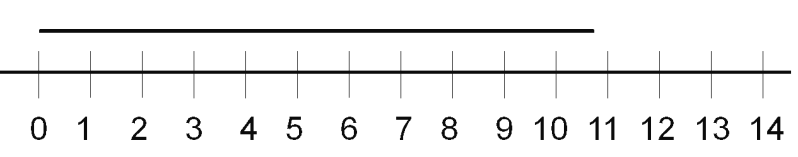
\includegraphics[scale=0.5]{figures_mvc/scalar_number_line}
\end{center}
A vector can therefore be represented as a \ti{directed} line segment, i.e., an arrow. As before, the length of the arrow will represent the magnitude of the vector. For example, if we wish to indicate a force of 2 pounds acting in the increasing \footnote{To represent a vector without ambiguity, when we specify the direction we must be sure to indicate the \ti{sense} of the vector. That is, in our present example, the word ``increasing'' denotes that we mean
\begin{center}
	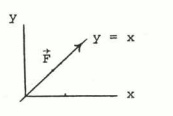
\includegraphics[scale=0.5]{figures_mvc/sense_1}
\end{center}
rather than
\begin{center}
	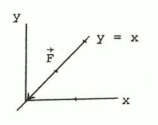
\includegraphics[scale=0.5]{figures_mvc/sense_2}
\end{center} In any diagram, it is therefore crucial to include the arrowhead to indicate the sense of the vector.} direction of the line $y=x$, we would represent it as the arrow ${\bf F}$.

\begin{center}
	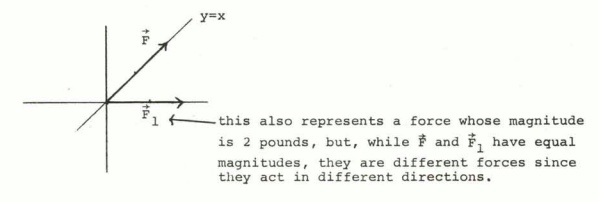
\includegraphics[scale=0.5]{figures_mvc/force_example}
\end{center}
The tail of the arrow is called the \ti{initial point} of the vector and the tip is called the \ti{terminal point}. 
\begin{center}
	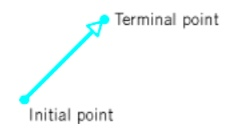
\includegraphics[scale=0.5]{figures_mvc/directed_line_segment}
\end{center}
We will denote a vector by boldface type, as in ${\bf v}$, and a scalar by lowercase italic type, as in $k$. When we want to indicate that a vector ${\bf v}$ has initial point $A$ and terminal point $B$, then we will write ${\bf v}=\overrightarrow{AB}$. \footnote{It is important to note that arrows are merely a convenient device to help us visualize vectors. That is, an arrow is a geometric representation of a vector, not the vector itself. Just as a number does not require the existence of a length, a vector require the existence of an arrow. Of course, once we have made this distinction, we may use vectors and arrows more or less interchangeably in the same way we use graphs and functions.}
\begin{center}
	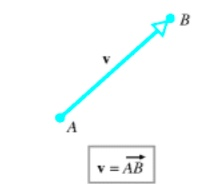
\includegraphics[scale=0.5]{figures_mvc/vAB}
\end{center}

\subsection{Vectors in coordinate systems}
As in analytic geometry, the use of coordinate systems give us powerful tools with which to perform concrete computations with vectors. Additionally, working with coordinates will allow us to consider geometric entities such as lines and planes in vector settings. 

\subsubsection{Coordinate correspondence}
In this section we describe the coordinate correspondence between three-dimensional Euclidean space, $\mathbb{E}^3$ (the three-dimensional space in which the axioms of Euclidean geometry hold), and three-dimensional Cartesian space $\mathbb{R}^3\equiv \{(x_1,x_2,x_3):x_i \in \mathbb{R} \text{ for } i=1,2,3\}$.

We begin with a line. A coordinate correspondence between a line $L$ and the real number system $\mathbb{R}$ is determined by choosing arbitrarily on $L$ a zero point $O$ and a unit point $Q$ distinct from $O$. Then to each point $X$ on $L$ is assigned the number $x$ such that $|x|$ is the distance from $O$ to $X$, measured in terms of the segment $OQ$ as the unit, and $x$ is positive or negative according to whether $X$ and $Q$ are on the same side of $O$ or on opposite sides. The mapping $X \mapsto x$ is the coordinate correspondence between $L$ and $\mathbb{R}$. 

We now set up a coordinate correspondence between $\mathbb{E}^3$ and $\mathbb{R}^3$. We first choose arbitrarily a zero point $O$ and three unit points $Q_1, Q_2,$ and $Q_3$ in such a way that the four points do not lie in a plane. Each of the unit points $Q_i$ determines a line $L_i$ through $O$ and a coordinate correspondence on this line, as defined above. The three lines $L_1, L_2$, and $L_3$ are called the \ti{coordinate axes}. Consider now any point $X$ in $\mathbb{E}^3$. The plane through $X$ parallel to $L_2$ and $L_3$ intersects $L_1$ at a point $X_1$, and therefore determines a number $x_1$, the coordinate of $X_1$ on $L_1$. Similarly, $X$ determines points $X_2$ on $L_2$ and $X_3$ on $L_3$ which have coordinates $x_2$ and $x_3$, respectively. Altogether, $X$ determines a triple
\begin{align*}
	{\bf x}=(x_1,x_2,x_3)
\end{align*} 
in $\mathbb{R}^3$, and we have thus defined a mapping $\theta:X \mapsto {\bf x}$ from $\mathbb{E}^3$ to $\mathbb{R}^3$. 

\begin{center}
	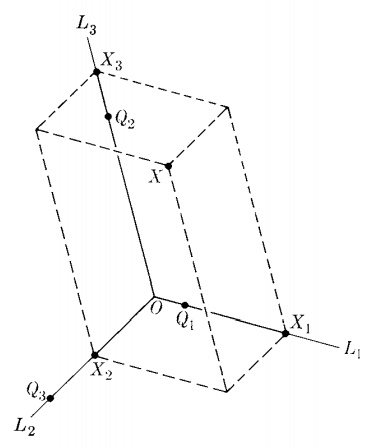
\includegraphics[scale=0.5]{figures_mvc/e3_r3}
\end{center}
We call $\theta$ the \ti{coordinate correspondence} defined by the axis system. Note that the unit point $Q_1$ on $L_1$ has the coordinate triple $(1,0,0)$, and similarly
\begin{align*}
	\theta(Q_2)&=(0,1,0), \\
	\theta(Q_3)&=(0,0,1).
\end{align*}

It is a fact that $\theta$ is a bijection from $\mathbb{E}^3$ to $\mathbb{R}^3$. The proof goes beyond the usual treatment of high school geometry, so we will simply accept this statement without proof.

\subsubsection{Cartesian coordinates}
\begin{defn}[Cartesian coordinates]
	The axis system in $\mathbb{E}^3$ is \ti{Cartesian} if the coordinate axes are mutually perpendicular and a common unit of distance (i.e., $|OQ_1|=|OQ_2|=|OQ_3|$) is used. The corresponding coordinates are called \ti{Cartesian coordinates}.
\end{defn}
A Cartesian coordinate system is shown below. \footnote{Cartesian coordinates are also often called \ti{rectangular coordinates} because the axes that define them meet at right angles.}
\begin{center}
	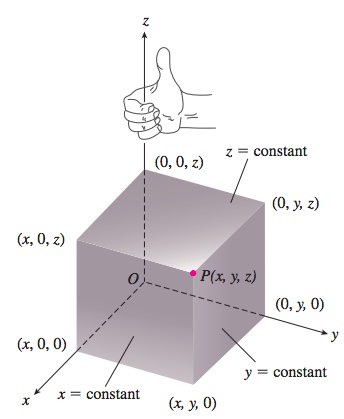
\includegraphics[scale=0.5]{figures_mvc/cartesian_coordinate_system}
\end{center}
The coordinate axes are labeled $x,y,$ and $z$, and are arranged such that if you take your right hand and curl your fingers from the positive $x$-axis toward the positive $y$-axis, your thumb points along the positive $z$-axis. Such a coordinate system is called \ti{right-handed}. \footnote{As you might have guessed, there are also left-handed coordinate systems. Choosing our coordinate system to be left- or right-handed is called choosing an \ti{orientation} for our coordinate system. We will discuss orientations more later. For now, just note that everything we do in the following could equivalently be formulated in terms of left-handed coordinate systems, so choosing a right-handed coordinate system for $\mathbb{E}^3$ is simply the standard convention.}

As discussed in the previous section, the coordinates of a point $P$ are the numbers at which the planes through $P$ perpendicular to the coordinate axes intersect these axes. These are labeled $\theta(P)=(x,y,z)$. 

Points on the $x$-axis have $y$- and $z$-coordinates equal to zero. That is, they have coordinates of the form $(x,0,0)$. Similarly points on the $y$- and $z$-axes have coordinates of the from $(0,y,0)$ and $(0,0,z)$, respectively.

The points in a plane perpendicular to the $x$-axis all have the same $x$-coordinate, $x_0$, this being the number at which the plane intersects that $x$-axis. The plane is then the set 
\begin{equation}
	P=\{(x,y,z) \in \mathbb{R}^3 : x=x_0\} 
\end{equation}
That is, the plane consists of all points having coordinates $(x_0,y,z)$, where $y$ and $z$ are any real numbers. The constraint $x=x_0$ is the equation of the plane perpendicular to the $x$-axis and intersecting it at $x_0$. Similar formulas hold for planes perpendicular to the $y$- and $z$-axes.

\begin{example}
The plane $x=2$ is the plane perpendicular to the $x$-axis at $x=2$. The plane $y=3$ is the plane perpendicular to the $y$-axis at $y=3$. The plane $z=5$ is the plane perpendicular to the $z$-axis at $z=5$. These planes are shown below, together with their intersection point $(2,3,5)$.
\end{example}

\begin{center}
	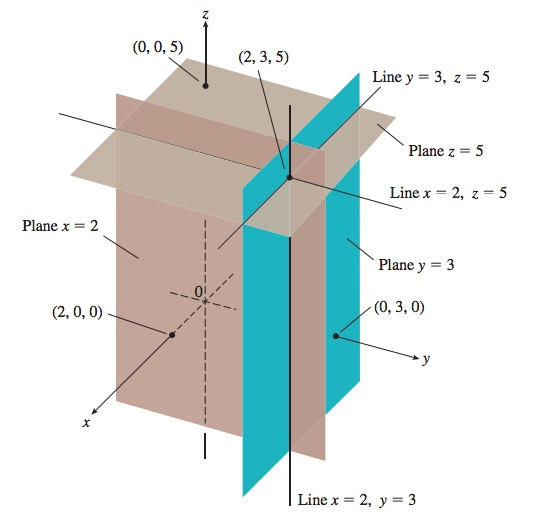
\includegraphics[scale=0.5]{figures_mvc/plane_235}
\end{center}

The planes $x=2$ and $y=3$ in the figure above intersect along a line parallel to the $z$-axis. This line is described by a pair of equations $L=\{(x,y,z) \in \mathbb{R}^3: x=2 \text{ and } y=3\}$.

\begin{exercise}
	Describe the other two lines of intersection in the figure above.
\end{exercise}

{\color{red} \flushleft {\bf Solution:}
The line running parallel to the $x$-axis is given by $$L_1=\{(x,y,z) \in \mathbb{R}^3: y=3 \text{ and } z=5\},$$ while the line running parallel to the $y$-axis is given by $$L_2=\{(x,y,z) \in \mathbb{R}^3: x=2 \text{ and } z=5\}.$$}

The three planes determined by the coordinate axes are the $xy$-plane, whose equation is $z=0$; the $yz$-plane, whose equation is $x=0$; and the $xz$-plane, whose equation is $y=0$. They meet at the origin, $(0,0,0)$.
	
The three coordinate planes $x=0, y=0,$ and $z=0$ divide space into eight cells called \ti{octants}. The octant in which the coordinates of all points are nonnegative is called the \ti{first octant}; there is no conventional numbering for the other seven octants.

\begin{exercise}
Write the coordinate equations and inequalities which define each of the following sets of points in space.
\begin{enumerate}[(a)]
	\item The half-space consisting of the points on and above the $xy$-plane.
	\item  This plane is parallel to the $yz$-plane and lying 3 units behind it.
	\item The second quadrant of the $xy$-plane.
	\item The first octant.
	\item The slab between the planes $y=-1$ and $y=1$, including these planes.
	\item The line in which the planes $y=-2$ and $z=2$ intersect.
\end{enumerate}	
\end{exercise}

{\color{red} \flushleft {\bf Solution:} 
\begin{enumerate}[(a)]
	\item $z \geq 0$,
	\item $x=-3$,
	\item $z=0, x \leq 0, z \geq 0$,
	\item $x \geq 0, y \geq 0, z \geq 0$,
	\item $-1 \leq y \leq 1$,
	\item $y=-2,z=2$.
\end{enumerate}}

\begin{exercise}
	What points $P(x,y,z)$ satisfy the equations
	\begin{align*}
		x^2+y^2=4 \text{ and }z=3?
	\end{align*}
\end{exercise}

{\color{red} \flushleft {\bf Solution:} These equations describe a circle of radius 2 lying in a plane parallel to the $xy$-plane and lying 3 units above it.}

\begin{center}
	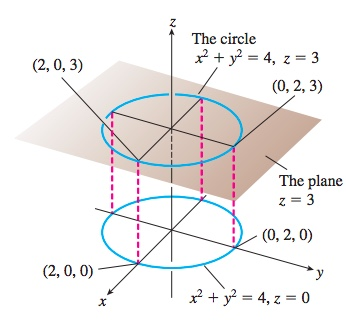
\includegraphics[scale=0.5]{figures_mvc/circle_z=3}
\end{center}

\subsubsection{Components of a vector}
Let us choose a Cartesian coordinate system for three-dimensional space. If a vector is positioned with its initial point at the origin, then the vector is completely determined by the coordinates of its terminal point.

\begin{center}
	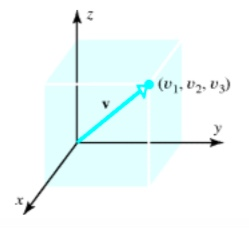
\includegraphics[scale=0.5]{figures_mvc/components}
\end{center}

\begin{defn}[Components of a vector]
	The coordinates of the terminal point of a vector ${\bf v}$ positioned with its initial point at the origin are called the \ti{components} of ${\bf v}$. We denote the components of a vector ${\bf v}$ by writing ${\bf v}=(v_1,v_2,v_3)$.
\end{defn}

\subsection{Vector arithmetic}
We have now defined a set of objects called vectors, which we visualize as arrows. To build a mathematical structure on this set, we need to define various rules and operations for working with vectors. As mathematicians, we are free to define any consistent set of rules and operations we like, and there are many possibilities.  Of course, our motivation for the introduction of vectors was to describe physical phenomena, and we will continue to take our motivations from physics in order to define a mathematical structure on the set of vectors.

\subsubsection{Equality of vectors}
The most basic rule is one which will allow us to determine when two vectors are equal. As we have taken a vector to have only two defining properties, namely its magnitude and direction, we will agree that
\begin{defn}[Equality of vectors]
Two vectors are equal if they have the same magnitude and direction.	
\end{defn}
In particular, this definition of equality means that if we have two distinct parallel line segments of the same length and we orient them with the same sense then these two vectors are equal.
\begin{center}
	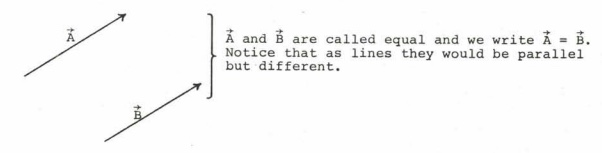
\includegraphics[scale=0.5]{figures_mvc/equal_vectors_new}
\end{center}
\begin{example}
A 2 second time interval and a 2 g mass are completely different physical quantities, their magnitude is exactly the same scalar, namely 2. Similarly, by our definition of equality of vectors, a velocity of 45 miles per hour along the increasing $y=x$ direction and a 45 $N$ force along the increasing $y=x$ direction are represented by exactly the same vector. \footnote{This is one of the reasons why mathematicians study abstract mathematical structures. Though one might have two sets of objects which look nothing alike, if they have the same mathematical structure, then any conclusions drawn about the first system hold \ti{verbatim} for the second system, simply by renaming the objects under consideration. This frees us from having to repeat the exact same mathematical computations for each concrete system we wish to consider; all we have to do is identify the mathematical structure of the set of objects we are studying, and then we know immediately that they behave exactly like every other set of objects which have the same mathematical structure.} 
\end{example}

\subsubsection{Vector addition}
Now that we know which vectors are distinct, our next step is to define operations on our set of vectors. The most basic operation is a \ti{binary operation}, which is a rule for combining any two vectors to produce a third. Exactly this kind operation can be studied in mechanics using a \ti{force table}.

\begin{center}
	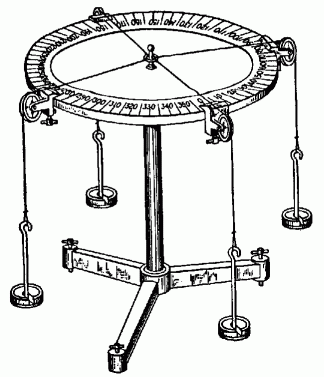
\includegraphics[scale=0.5]{figures_mvc/force_table_experiment_2}
\end{center}

In a force table experiment, strings are tied to a metal ring which is positioned at the center of the table. The strings are then suspended over pulleys which are fixed at known angles, and known masses hung from the ends of the strings. The pull of gravity on a given mass creates tension in the string which pulls on the washer. 

In an experiment in which \ti{two} strings are tied to the washer, the tension in each string gives rise to two forces pulling on the washer in different directions. However, the washer ultimately accelerates in a single direction, which is the direction of the \ti{net} (or \ti{total}) force acting on the washer. The rule for combining the two tension force vectors to produce the net force vector is exactly the binary operation we seek to define. Then, since we already have a definition which tells us when two vectors are equal, this rule will apply to \ti{all} vectors, whether they are forces, velocities, momenta, or any other type of vectors. 

To determine the net force, a third string is connected to the washer with pulley positioned and mass chosen so that the washer is in \ti{static equilibrium} (i.e., it does not move at all under the influence of these three forces). This vector is called the \ti{equilibrant} vector. By Newton's third law, the net force vector (also called the \ti{resultant} vector) is then the \ti{opposite} of the equilibrant vector, that is, it has the same magnitude and is directed along the same line, but with the opposite sense.

\begin{center}
	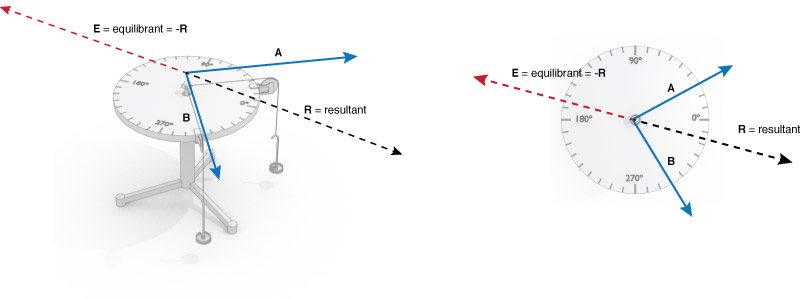
\includegraphics[scale=0.5]{figures_mvc/force-table-equi-res}
\end{center}

 We therefore define the \ti{sum} of two vectors as  
 
 \begin{defn}[Vector addition]
 	The \ti{sum} ${\bf v}+{\bf w}$ of two vectors ${\bf v}$ and ${\bf w}$ is the resultant vector of ${\bf v}$ and ${\bf w}$.
 \end{defn}
Note that when the two tension forces are along the \ti{same} direction (e.g., just add another mass on the same string), the resultant vector points in this same direction and has magnitude given by the sum of the magnitudes of the two tension vectors, and hence the addition of ${\bf v}$ and ${\bf w}$ reduces to addition of ordinary numbers in this special case. This is why we have decided to call this binary operation \ti{addition} and to continue to denote it by $+$; that is, it is a \ti{generalization} of ordinary addition. \footnote{To be completely rigorous and unambiguous, we should technically use some new symbol for this binary operation, such as ${\bf v}*{\bf w}$. However, it is standard practice to use the same symbol in such situations as it is conceptually useful to keep in mind the fact that this is a generalization of another operation.}
 
In terms of our geometric representation of vectors, the magnitude and direction of ${\bf v}+{\bf w}$ is determined as follows: Since the location of a vector is of no consequence (by our definition of equality of vectors), we may position the two vectors so that their initial points coincide. Then ${\bf v}$ and ${\bf w}$ form adjacent sides of a parallelogram, and the vector ${\bf v}+{\bf w}$ is the diagonal of the parallelogram, directed from the common initial point of ${\bf v}$ and ${\bf w}$ to the opposite vertex of the parallelogram, as shown below.	
\begin{center}
	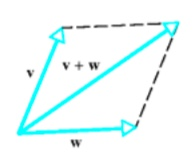
\includegraphics[scale=0.5]{figures_mvc/parallelogram_rule}
\end{center}
This is called the \ti{parallelogram rule} for vector addition. Since the opposite sides of a parallelogram are congruent and parallel, we can equivalently view ${\bf v}+{\bf w}$ as the result of positioning the initial point of ${\bf w}$ at the terminal point of ${\bf v}$ and drawing the arrow connecting the initial point of ${\bf v}$ to the terminal point of ${\bf w}$.

\begin{center}
	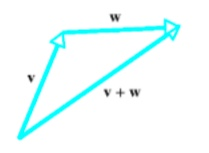
\includegraphics[scale=0.5]{figures_mvc/tip_to_tail}
\end{center}
This is called the \ti{triangle rule} or \ti{``tip to tail" rule} for vector addition. These two points of view are related by \ti{parallel translation}. To go from the first point of view to the second, we translate the initial point of ${\bf w}$ along ${\bf v}$, keeping ${\bf w}$ parallel to its original direction at all times. Accordingly, ${\bf v}+{\bf w}$ is also called the \ti{translation of ${\bf w}$ by ${\bf v}$}.
\begin{center}
	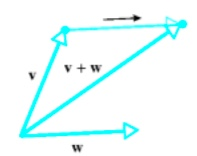
\includegraphics[scale=0.5]{figures_mvc/translation_of_v_by_w}
\end{center}
Let us emphasize once more that nothing forced us to choose this definition of vector addition, but by making this choice we are sure that our definition has at least one real interpretation, namely as the resultant vector in mechanics.

Let us now examine the properties of vector addition. Recall that the addition operation defined on the set of real numbers satisfies the following properties:
\begin{enumerate}[(a)]
	\item Commutativity: $x+y=y+x$ for all $x,y \in \mathbb{R}$.
	\item Associativity: $(x+y)+z=x+(y+z)$ for all $x,y,z \in \mathbb{R}$.
	\item Existence of an additive identity: $\mathbb{R}$ contains an element 0 such that $0+x=x$ for every $x \in \mathbb{R}$.
	\item Existence of additive inverses: For every $x \in \mathbb{R}$, there exists and element $y \in \mathbb{R}$ such that $x+y=0$.
\end{enumerate}
Let us use our definition of vector addition to consider each of these in turn.

\begin{prop}[Vector addition is commutative]
	Vector addition is commutative. That is, 
	\begin{align*}
		{\bf v}+{\bf w}={\bf w}+{\bf v}
	\end{align*}
	for any two vectors ${\bf v}$ and ${\bf w}$.
\end{prop}

\begin{pf}
	We see from the two diagrams below that the translation of ${\bf w}$ by ${\bf v}$ is the same vector as the translation of ${\bf v}$ by ${\bf w}$.
\begin{center}
	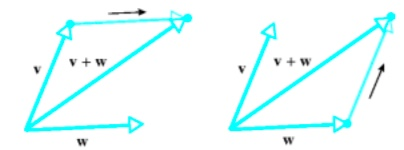
\includegraphics[scale=0.5]{figures_mvc/equivalence_of_vector_addition}
\end{center}

\end{pf}

\begin{prop}[Vector addition is associative]
	Vector addition is associative. That is, for any three vectors ${\bf u}, {\bf v},$ and ${\bf w}$, we have
	\begin{align*}
		{\bf u}+({\bf v}+{\bf w})=({\bf u}+{\bf v})+{\bf w}
	\end{align*}
We therefore denote both expressions by ${\bf u}+{\bf v}+{\bf w}$. 
\end{prop}

\begin{pf}
One can construct ${\bf u}+{\bf v}+{\bf w}$ by placing the vectors ``tip to tail" in succession and then drawing the vector from the initial point of ${\bf u}$ to the terminal point of ${\bf w}$. One can easily verify associativity from this construction, as shown below.
\end{pf}

\begin{center}
	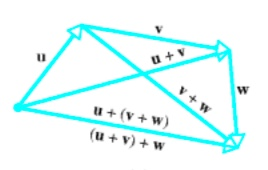
\includegraphics[scale=0.5]{figures_mvc/associativity_of_vector_addition}
\end{center}

The tip-to-tail method also makes it evident that if ${\bf u}, {\bf v},$ and ${\bf w}$ have a common initial point, then ${\bf u}+{\bf v}+{\bf w}$ is the diagonal of the parallelepiped that has the three vectors as adjacent sides.

\begin{center}
	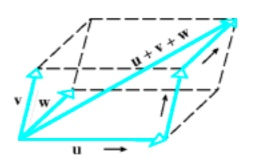
\includegraphics[scale=0.5]{figures_mvc/volume_of_parallelepiped_vectors}
\end{center}

\begin{cor}
The sum ${\bf v}_1+{\bf v}_2+\cdots + {\bf v}_k$ is independent of how the expression is bracketed.	
\end{cor}

\begin{pf}
As in the case of real numbers, the proof follows by induction on $k$. We will not repeat this here. \footnote{Of course, none of the proofs just presented are really proofs at all, since drawing pictures is not an acceptable substitute for airtight logic. For now, take them as plausibility arguments. We will prove these propositions rigorously in the next section.}	
\end{pf}

Let us now check whether there is a vector which plays the role of an additive identity. That is, given any vector ${\bf b}$, is there a vector ${\bf 0}$ such that ${\bf b}+{\bf 0}={\bf b}$? Let us suppose there is such a vector ${\bf 0}$ and denote its magnitude by $r$. Let us now add ${\bf 0}$ to ${\bf b}$ by the tip-to-tail method. Since ${\bf 0}$ has magnitude $r$, ${\bf b}+{\bf 0}$ must lie on a circle of radius $r$ centered on the tip of ${\bf b}$. However, the condition ${\bf b}+{\bf 0}={\bf b}$ means that ${\bf b}+{\bf 0}$ must have the same magnitude and direction as ${\bf b}$, and there is no point on the circle for which this is true. This shows that there is no such vector ${\bf 0}$ with nonzero length. 
\begin{center}
	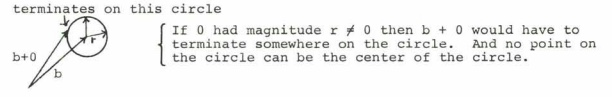
\includegraphics[scale=0.5]{figures_mvc/b_plus_zero_circle}
\end{center}

Thus, any vector of magnitude zero satisfies the requirement to serve as ${\bf 0}$, independently of direction. Now, for the real numbers, $0$ is unique, since if there are two numbers $0$ and $0'$ such that $x+0=x$ and $x+0'=x$ for all $x \in \mathbb{R}$, then $0=0+0'=0'$. However, our definition of equality of vectors says that two vectors of zero magnitude but different directions are not equal. Thus, if we want the zero vector to be unique, we must agree that we do not distinguish between two vectors of zero magnitude, even if they have different directions. This agrees with our geometric intuition, since a line segment of zero length is a point, which has no direction. Thus, with our modified definition of equality of vectors 

\begin{defn}[Equality of vectors ']
\begin{enumerate}[(1)] \hspace{10cm}
	\item Two nonzero vectors are equal if they have the same magnitude and direction.
	\item Any two vectors of zero magnitude are equal, even if their directions are different.
\end{enumerate}	
\end{defn}
and our definition of the zero vector
\begin{defn}[The zero vector]
	The zero vector, ${\bf 0}$, is any vector of zero magnitude.
\end{defn}
then ${\bf a}+{\bf b}$ is defined for \ti{any} two vectors ${\bf a}$ and ${\bf b}$, even if one is zero, and the zero vector ${\bf 0}$ is unique. \footnote{Note from our definition that the zero vector ${\bf 0}$ is not a single vector, but is actually a collection of vectors; namely, ${\bf 0}$ is the \ti{equivalence class} of all vectors with zero magnitude.}

Finally, we want to investigate whether, given any vector ${\bf a}$, we can find another vector ${\bf b}$ such that ${\bf a}+{\bf b}={\bf 0}$, where ${\bf 0}$ here denotes the zero vector. Since the zero vector has no length and since we add vectors from ``tip to tail", it follows that if ${\bf a}+{\bf b}={\bf 0}$, then the tail of ${\bf a}$ and the tip of ${\bf b}$ must coincide. This in turn means that ${\bf b}$ must have the same magnitude as ${\bf a}$ but opposite direction (directed along the same line, but with the opposite sense).  
\begin{center}
	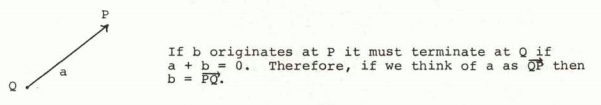
\includegraphics[scale=0.5]{figures_mvc/a_plus_b_equals_zero}
\end{center}
In other words, if we wish for vector addition to have the same structure as that of numerical addition, we \ti{must} define 
\begin{defn}[Inverse of a vector]
The additive inverse of ${\bf a}$ to be the vector which has the same magnitude, but opposite direction. 	
\end{defn}
In analogy with the equation $x+(-x)=0$ for real numbers, we denote the additive inverse of ${\bf a}$ by $-{\bf a}$, so that ${\bf a}+(-{\bf a})={\bf 0}$ for any vector ${\bf a}$. We may again agree, as in the case of numerical addition, to abbreviate ${\bf a}-{\bf b}$ as ${\bf a}-{\bf b}$, which allows us to define vector subtraction:

\begin{defn}[Vector subtraction]
	The difference ${\bf a}-{\bf b}$ of two vectors ${\bf a}$ and ${\bf b}$ is the sum
	\begin{align*}
		{\bf a}-{\bf b}={\bf a}+(-{\bf b}).
	\end{align*}
\end{defn}
From this definition, we may view vector subtraction geometrically as follows: To form ${\bf a}-{\bf b}$,
\begin{enumerate}[(1)]
	\item Obtain $(-{\bf b})$ from ${\bf b}$ by reversing the direction of ${\bf b}$.
	\item Add ${\bf a}$ and $(-{\bf b})$ in the usual way, by placing the tail of $(-{\bf b})$ at the tip of ${\bf a}$. \footnote{Like numerical subtraction, vector subtraction is \ti{not} commutative, so the order matters here.}
\end{enumerate}

\begin{center}
	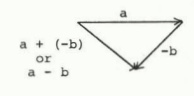
\includegraphics[scale=0.5]{figures_mvc/a_minus_b}
\end{center}

\begin{exercise}
Consider adding vectors ${\bf a}$ and ${\bf b}$ tail-to-tail, as shown below
	\begin{center}
		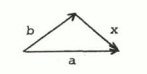
\includegraphics[scale=0.5]{figures_mvc/b_plus_x_equals_a}
	\end{center}
	Show that ${\bf x}={\bf a}-{\bf b}$. This gives another view of vector subtraction which is very useful computationally.
\end{exercise}

{\color{red} \flushleft {\bf Solution:}
We see from the tip-to-tail rule, that ${\bf b}+{\bf x}={\bf a}$. Adding $(-{\bf b})$ to both sides of this equation and using associativity gives ${\bf x}={\bf a}-{\bf b}$.}

The previous exercise shows that, if ${\bf a}$ and ${\bf b}$ are any two vectors and we wish to find ${\bf a}-{\bf b}$, we place the two vectors tail-to-tail and ${\bf a}-{\bf b}$ is then the vector which extends from the tip of ${\bf b}$ to the tip of ${\bf a}$.

We have just shown that our definition of vector addition satisfies the same properties as numerical addition. That is, the additive structures are exactly the same for vectors as for numbers. Therefore, any results that hold for numbers also hold for vectors, for exactly the same reasons. For example,

\begin{thm}[Cancellation law]
	If ${\bf a}, {\bf b},$ and ${\bf c}$ are vectors such that ${\bf a}+{\bf b}={\bf a}+{\bf c}$, then ${\bf b}={\bf c}$. 
\end{thm}

\begin{pf}
The proof is exactly the same as for numbers, with the word ``vector" substituted for ``number".
\end{pf}

This is one illustration of the power of mathematical structure; namely, it is only the rules which determine how the various objects are related that are important, not the objects themselves.

\subsubsection{Scalar multiplication}
In physics, we observe that an unbalanced force on a body causes an acceleration in the direction of the force. It is also observed that the magnitude of acceleration of different bodies, when subjected to the same force, varies according to their mass. These observations are formalized in Newton's second law of motion
\begin{equation}
	{\bf F}=m{\bf a}.
\end{equation}
On the right side of this equation, we see a new operation: the product of a scalar and a vector. Due to the fundamental nature of Newton's second law, if we want to build a mathematical structure which is capable of describing nature, we should include this operation.

\begin{defn}[Scalar multiplication]
The \ti{scalar multiple} of the vector ${\bf v}$ by the scalar ${\bf k}$ is the vector ${\bf w}=k{\bf v}$. The length of ${\bf w}$ is $|k|$ times the length of ${\bf v}$. If $k>0$, ${\bf w}$ points in the same direction as ${\bf v}$, while if $k<0$, ${\bf w}$ points in the direction of $-{\bf v}$. If $k=0$ or ${\bf v}={\bf 0}$, then we defined $k{\bf v}$ to be ${\bf 0}$.
\end{defn}

\begin{example}
The vector $2{\bf v}$ has the same direction as ${\bf v}$ but twice its length, while $-2{\bf v}$ is oppositely directed to ${\bf v}$ and twice its length.	
\end{example}

\begin{prop}[Properties of scalar multiplication]
For any scalars $c,d$ and vectors ${\bf v}, {\bf w}$,
	\begin{enumerate}[(a)]
		\item $(c+d){\bf v}=c{\bf v}+d{\bf v}$,
		\item $c({\bf v}+{\bf w})=c{\bf v}+c{\bf w}$,
		\item $(dc){\bf v}=c(d{\bf v})$,
		\item 1{\bf v}={\bf v},
		\item 0{\bf v}={\bf 0},
		\item $(-1){\bf v}=-{\bf v}$.
	\end{enumerate}
\end{prop}

\begin{pf}
	\fixme{Add proof. Does 1 depend on the triangle inequality?}
\end{pf}


\subsubsection{Norm of a vector}
A \ti{norm} is a function which takes a vector as input and returns its magnitude. Here, we review the standard \ti{Euclidean norm}, which is given in terms of the Cartesian coordinates of a vector. 
\begin{defn}[Norm of a vector]\label{def:length_of_a_vector}
	The \ti{norm} of a vector ${\bf v}$, denoted $||{\bf v}||$, is given in terms of its Cartesian coordinates by
	\begin{align*}
		||{\bf v}||=\sqrt{v_1^2+v_2^2+v_3^2}.
	\end{align*}
\end{defn}

\begin{pf}
This formula follows directly from the Pythagorean theorem. In the diagram below,
\begin{center}
	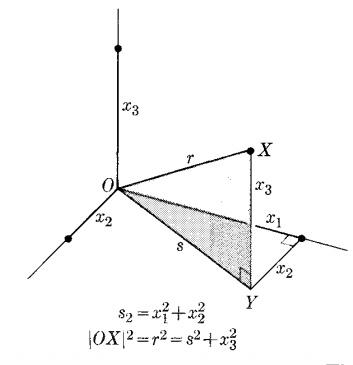
\includegraphics[scale=0.5]{figures_mvc/euclidean_norm}
\end{center}	
we see from the right triangle in the $x_1x_2$-plane that that $s^2=x_1^2+x_2^2$. Then, from triangle $XYO$, we have $r^2=s^2+x_3^2=x_1^2+x_2^2+x_3^2$.
\end{pf}

\begin{prop}[Norm properties]
	For any scalar $a$ and any vectors ${\bf v}$ and ${\bf w}$,
	\begin{enumerate}[(1)]
		\item $||{\bf u}+{\bf v}||\leq ||{\bf u}|| + ||{\bf v}||$ (triangle inequality)
		\item $||a{\bf v}||=|a| \ ||{\bf v}||$ (homogeneity)
		\item If $||{\bf v}||=0$, then ${\bf v}={\bf 0}$ (positive-definite)
	\end{enumerate}
\end{prop}

\begin{pf}
Verify these for the Euclidean norm. More generally, we take these to be the defining properties of a norm.
\end{pf}

\begin{defn}[Unit vector]
	A \ti{unit vector} is a vector of unit length. That is, a vector ${\bf v}$ such that $||{\bf v}||=1$.
\end{defn}

\begin{prop}[Normalizing a vector]
	If ${\bf v}\neq 0$, then ${\bf v}/||{\bf v}||$ is a unit vector in the direction of ${\bf v}$. The unit vector ${\bf v}/||{\bf v}||$ is often denoted ${\bf \hat{v}}$ and the process of forming ${\bf \hat{v}}$ from ${\bf v}$ is called \ti{normalizing} ${\bf v}$.
\end{prop}

\begin{pf}
Since ${\bf v}\neq 0$, $||{\bf v}|| \neq 0$, so we can multiply ${\bf v}$ by $1/||{\bf v}||$. Computing the length of $||\frac{{\bf v}}{||{\bf v}||}||$, we see that 
\begin{align*}
	||\frac{{\bf v}}{||{\bf v}||}||&=\frac{||{\bf v}||}{||{\bf v}||}=1,
\end{align*} 
hence ${\bf v}/||{\bf v}||$ is a unit vector. Since ${\bf v}/||{\bf v}||$ is a scalar multiple of ${\bf v}$ (by $k=1/||{\bf v}||$) it is parallel to ${\bf v}$.
\end{pf}

\begin{example}
	We can express any nonzero vector ${\bf v}$ as a product of its magnitude and direction by means of the formula
	\begin{align*}
		{\bf v}=||{\bf v}||\frac{{\bf v}}{||{\bf v}||}.
	\end{align*}
	For example, taking ${\bf v}=(1,-2,3)$,
	\begin{align*}
		||{\bf v}||=\sqrt{1^2+(-2)^2+3^2}=\sqrt{14}
	\end{align*}
	and thus
	\begin{align*}
		{\bf v}=\sqrt{14}(\frac{1}{\sqrt{14}},\frac{-2}{\sqrt{14}},\frac{3}{\sqrt{14}}).
	\end{align*}
\end{example}


\begin{defn}[Standard unit vectors]
	 The \ti{standard unit vectors} for $\mathbb{E}^3$ are the vectors
	\begin{align*}
		{\bf e}_1&=(1,0,0), \\
		{\bf e}_2&=(0,1,0), \\
		{\bf e}_3&=(0,0,1). \\
	\end{align*}
These vectors are unit vectors pointing along the $x$-, $y$-, and $z$-axes, respectively. \footnote{The standard unit vectors $({\bf e}_1,{\bf e}_2,{\bf e}_3)$ are also commonly denoted as $({\bf i}, {\bf j}, {\bf k})$ or $({\bf \hat{x}}, {\bf \hat{y}}, {\bf \hat{z}})$.}	
\end{defn}
Using the standard unit vectors, we may write the vector ${\bf v}=(v_1,v_2,v_3)$ as $${\bf v}=v_1{\bf e}_1+v_2{\bf e}_2+v_3{\bf e}_3.$$

\begin{prop}[Vector operations in coordinates]
	Let ${\bf v}=(v_1,v_2,v_3)$ and ${\bf w}=(w_1,w_2,w_3)$ be vectors and $k$ a scalar. Then
	\begin{align*}
		{\bf v}+{\bf w}&=(v_1+w_1,v_2+w_2,v_3+w_3), \\
		{\bf v}-{\bf w}&=(v_1-w_1,v_2-w_2,v_3-w_3), \\
		k{\bf v}&=(kv_1,kv_2,kv_3).
	\end{align*}
\end{prop}

\begin{pf}
These formulas can be seen by examining the following diagrams.
\begin{center}
	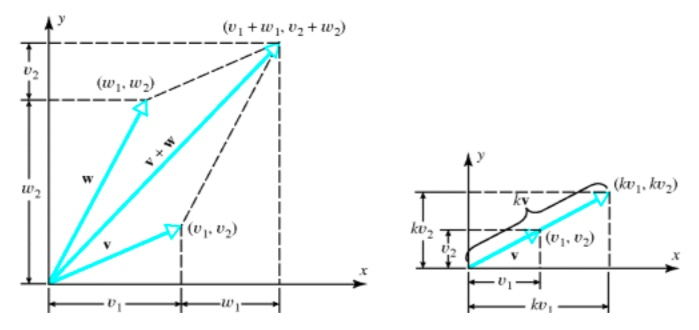
\includegraphics[scale=0.5]{figures_mvc/vector_operations}
\end{center}	
\end{pf}

\begin{prop}[Vector from one point to another]\label{prop:vector_from_one_point_to_another}
	The vector from $P_1(x_1,y_1,z_1)$ to $P_2(x_2,y_2,z_2)$ is given by
	\begin{align*}
		\overrightarrow{P_1P_2}=(x_2-x_1,y_2-y_1,z_2-z_1).
	\end{align*}
\end{prop}

\begin{pf}
From the figure below, 
\begin{center}
	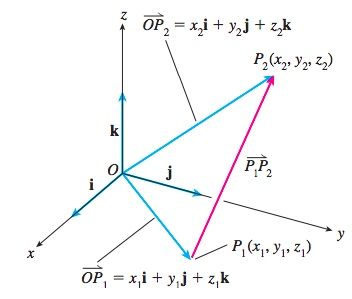
\includegraphics[scale=0.5]{figures_mvc/P1P2}
\end{center}

we see that $\overrightarrow{OP_1}+\overrightarrow{P_1P_2}=\overrightarrow{OP_2}$, and therefore
\begin{align*}
	\overrightarrow{P_1P_2}&=\overrightarrow{OP_2}-\overrightarrow{OP_1} \\
	&=(x_2,y_2,z_2)-(x_1,y_1,z_1) \\
	&=(x_2-x_1,y_2-y_1,z_2-z_1).
\end{align*}	
\end{pf}

\begin{cor}[Distance between two points]
	The distance between two points $P_1(x_1,y_1,z_2)$ and $P_2(x_2,y_2,z_2)$ is given by
	\begin{align*}
		||\overrightarrow{P_1P_2}||=\sqrt{(x_2-x_1)^2+(y_2-y_1)^2+(z_2-z_1)^2}.
	\end{align*}
\end{cor}

\begin{pf}
	This formula follows immediately from Prop. \ref{prop:vector_from_one_point_to_another} and Def. \ref{def:length_of_a_vector}.
\end{pf}

\begin{exercise}
\begin{enumerate}[(a)]
	\item Find the components of the vector $\overrightarrow{P_1P_2}$ with initial point $P_1(2,-1,4)$ and terminal point $P_2(7,5,-8)$.
	\item Find the distance between $P_1(2,-1,4)$ and $P_2(7,5,-8)$.
\end{enumerate}	
\end{exercise}

{\color{red} \flushleft {\bf Solution:} 
\begin{enumerate}[(a)]
	\item The components of $\overrightarrow{P_1P_2}$ are given by
	\begin{align*}
		\overrightarrow{P_1P_2}=(7-2,5-(-1),-8-4)=(5,6,-12)
	\end{align*}
	\item The distance between $P_1$ and $P_2$ is 
	\begin{align*}
		||\overrightarrow{P_1P_2}||=\sqrt{5^2+6^2+(-12)^2}=\sqrt{205}.
	\end{align*}
\end{enumerate}}

\begin{exercise}
Find a unit vector in the direction of the vector from $P_1(1,0,1)$ to $P_2(3,2,0)$.
\end{exercise}

{\color{red} \flushleft {\bf Solution:}
We find $\overrightarrow{P_1P_2}$ and normalize:
\begin{align*}
	\overrightarrow{P_1P_2}&=(3-1,2-0,0-1)=(2,2,-1), \\
	||\overrightarrow{P_1P_2}||&=\sqrt{2^2+2^2+(-1)^2}=3, \\
\end{align*}
and therefore the desired unit vector is given by
\begin{align*}
	\frac{\overrightarrow{P_1P_2}}{||\overrightarrow{P_1P_2}||}=(\frac{2}{3},\frac{2}{3},-\frac{1}{3}).
\end{align*}}

\begin{exercise}
Find a vector 6 units long in the direction of ${\bf v}=(2,2,-1)$.	
\end{exercise}

{\color{red} \flushleft {\bf Solution:}
The vector we want is 
\begin{align*}
6\frac{{\bf v}}{||{\bf v}||}=6\frac{(2,2,-1)}{\sqrt{2^2+2^2+(-1^2)}}=6\frac{(2,2,-1)}{3}=(4,4,-2).	
\end{align*}
}

\begin{exercise}
	A sphere of radius $r$ centered at $(x_0,y_0,z_0)$ is the set of all points in $\mathbb{R}^3$ equidistant from $(x_0,y_0,z_0)$. Find the equation of the sphere.
\end{exercise}

{\color{red} \flushleft {\bf Solution:}
Let $(x,y,z)$ be an arbitrary point in $\mathbb{R}^3$. The vector from $P_1(x_0,y_0,z_0)$ to $P_2(x,y,z)$ is then
\begin{align*}
	\overrightarrow{P_1P_2}=(x-x_0,y-y_0,z-z_0).
\end{align*}
The length of $\overrightarrow{P_1P_2}$ is then
\begin{align*}
	||\overrightarrow{P_1P_2}||=\sqrt{(x-x_0)^2+(y-y_0)^2+(z-z_0)^2}.
\end{align*}
By definition, the sphere is the set of all $(x,y,z)$ such that $||\overrightarrow{P_1P_2}||=r$. Squaring both sides to get rid of the awkward square root gives the standard equation of a sphere:
\begin{align*}
	(x-x_0)^2+(y-y_0)^2+(z-z_0)^2=r^2.
\end{align*}}

\begin{prop}[Midpoint formula]
	The midpoint $M$ of the line segment joining points $P_1(x_1,y_1,z_1)$ and $P_2(x_2,y_2,z_2)$ is the point
	\begin{align*}
		\left(\frac{x_1+x_2}{2},\frac{y_1+y_2}{2},\frac{z_1+z_2}{2}\right).
	\end{align*}
\end{prop}

\begin{pf}
From the figure below, we see that
\begin{align*}
	\overrightarrow{OM}&=\overrightarrow{OP_1}+\frac{1}{2}\overrightarrow{P_1P_2} \\
	&=\overrightarrow{OP_1}+\frac{1}{2}(\overrightarrow{OP_2}-\overrightarrow{OP_1}) \\
	&=\frac{1}{2}(\overrightarrow{OP_2}+\overrightarrow{OP_1}) \\
	&=\left(\frac{x_1+x_2}{2},\frac{y_1+y_2}{2},\frac{z_1+z_2}{2}\right).
\end{align*}
\begin{center}
	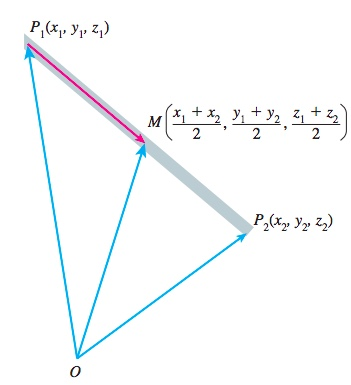
\includegraphics[scale=0.5]{figures_mvc/midpoint_formula}
\end{center}	
\end{pf}

\begin{exercise}
Find the midpoint of the segment joining $P_1=(3,-2,0)$ and $P_2(7,4,4)$.	
\end{exercise}

{\color{red} \flushleft {\bf Solution:}
The midpoint is the point
\begin{align*}
	\left(\frac{3+7}{2},\frac{-2+4}{2},\frac{0+4}{2}\right)=(5,1,2).
\end{align*}}

\subsubsection{The dot product}
Two nonzero vectors ${\bf u}$ and ${\bf v}$ positioned so that their initial points coincide determine an angle $\theta \in [0,\pi]$, which is the angle between the two vectors.
\begin{center}
	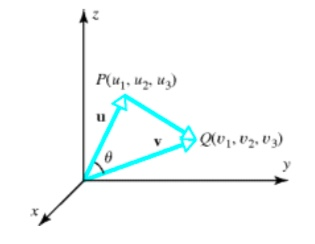
\includegraphics[scale=0.5]{figures_mvc/angle_uv}
\end{center}
Note that the information about $\theta$ is encoded in ${\bf u}-{\bf v}$, since if we fix the magnitudes of ${\bf u}$ and ${\bf v}$ and open the angle, then ${\bf u}-{\bf v}$ will also change. The fundamental relation satisfied by ${\bf u}, {\bf v}$ and $\theta$ is the law of cosines, which says that if ${\bf w}={\bf u}-{\bf v}$, then
\begin{equation}\label{eq:law_of_cosines}
	||{\bf w}||^2=||{\bf u}||^2+||{\bf v}||^2-2||{\bf u}|| \ ||{\bf v}||\cos \theta. 
\end{equation}
Let us make the following definition.
\begin{defn}[Dot product]
	The \ti{dot product} of two vectors ${\bf u}$ and ${\bf v}$ is defined by
	\begin{equation}\label{eq:dot_product_def}
		{\bf u}\cdot {\bf v}=||{\bf u}|| \ ||{\bf v}||\cos\theta.
	\end{equation} 
\end{defn}
The angle between two vectors ${\bf u}$ and ${\bf v}$ is then given by
\begin{equation}\label{eq:angle_uv}
	\theta=\cos^{-1}\left(\frac{{\bf u}\cdot {\bf v}}{||{\bf u}|| \ ||{\bf v}||}\right),
\end{equation}	
and we see that
\begin{itemize}
	\item $\theta$ is acute if ${\bf u} \cdot {\bf v} > 0$.
	\item $\theta$ is obtuse if ${\bf u} \cdot {\bf v} < 0$.
	\item $\theta$ is right if ${\bf u} \cdot {\bf v} = 0$.
\end{itemize}

Since the dot product takes as input two vectors and returns a scalar, it is also called the \ti{scalar product}. Note that from Eq. \eqref{eq:law_of_cosines}, we can write ${\bf u}\cdot {\bf v}$ in terms of magnitudes only, as 
\begin{equation}\label{eq:dot_product_magnitudes}
	{\bf u}\cdot {\bf v}=\frac{||{\bf u}||^2+||{\bf v}||^2-||{\bf u}-{\bf v}||^2}{2}.
\end{equation}
Note that this equation holds in \ti{all} coordinate systems. However, it takes a particularly simple form in Cartesian coordinates. Writing out the norm of each vector in terms of its components gives

\begin{align*}
	{\bf u}\cdot {\bf v}&=\frac{u_1^2+u_2^2+u_3^2+v_1^2+v_2^2+v_3^2-(u_1-v_1)^2-(u_2-v_2)^2-(u_3-v_3)^2}{2}
\end{align*}
Expanding the binomials and cancelling like terms, we find
\begin{equation}
	{\bf u}\cdot {\bf v}=u_1v_1+u_2v_2+u_3v_2.
\end{equation}

\begin{exercise}
Compute the angle between the vectors ${\bf u}=(0,0,3)$ and ${\bf v}=(\sqrt{2},0,\sqrt{2})$.	
\end{exercise}

{\color{red} \flushleft {\bf Solution:} The angle between these vectors is
\begin{align*}
	\theta=\cos^{-1}\left(\frac{0(\sqrt{2}+0(0)+3(\sqrt{2}))}{3(2)}\right)=\cos^{-1}\left(\frac{1}{\sqrt{2}}\right)=\frac{\pi}{4}.
\end{align*}}

\begin{exercise}
	Find the angle between a diagonal of a cube and one of its edges.
\end{exercise}

{\color{red} \flushleft {\bf Solution:}
Let $s$ be the length of an edge and place the cube in the first octant so that one vertex is at the origin and two edges are along the $x$- and $y$-axes.
\begin{center}
	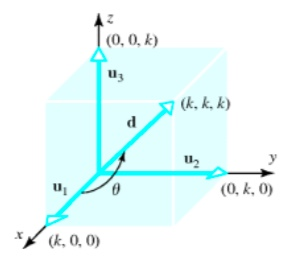
\includegraphics[scale=0.5]{figures_mvc/cube_coordinates}
\end{center}
If we let ${\bf u}_1=(s,0,0), {\bf u}_1=(0,s,0)$, and ${\bf u}_3=(0,0,s)$, then the vector
\begin{align*}
	{\bf d}=(s,s,s)={\bf u}_1+{\bf u}_2+{\bf u}_3
\end{align*}
is a diagonal of the cube. The angle between ${\bf d}$ and ${\bf u}_1$ is 
\begin{align*}
	\theta &=\cos^{-1}\left(\frac{{\bf u}_1 \cdot {\bf d}}{||{\bf u}_1 || \ || {\bf d}||}\right) \\
	&=\cos^{-1}\left(\frac{s^2}{(s)(\sqrt{3s^2})}\right)  \\
	&=\cos^{-1}\left(\frac{1}{\sqrt{3}}\right) \\
	&\approx 54.74^\circ.
\end{align*}
}

\begin{prop}[Properties of the dot product]
	Let ${\bf a}, {\bf b}, {\bf c}, {\bf d}$ be vectors and $k$ any scalar. Then 
	\begin{enumerate}[(1)]
		\item ${\bf a}\cdot {\bf b}={\bf b} \cdot {\bf a}$
		\item $(k {\bf a})\cdot {\bf b}={\bf a}\cdot (k{\bf b})=k({\bf a}\cdot {\bf b})$
		\item ${\bf a}\cdot ({\bf b}+{\bf c})={\bf a}\cdot {\bf b}+{\bf a}\cdot {\bf c}$
		\item $({\bf a}+{\bf b})\cdot {\bf a}={\bf a}\cdot {\bf c}+{\bf b}\cdot {\bf c}$
		\item $({\bf a}+{\bf b})\cdot ({\bf c}+{\bf d})={\bf a}\cdot {\bf c}+{\bf a}\cdot {\bf d}+{\bf b}\cdot {\bf c}+{\bf b}\cdot {\bf d}$
		\item ${\bf a} \cdot {\bf a}=||{\bf a}||^2$
	\end{enumerate}
\end{prop}

\begin{pf}
Each of these can be proved by writing out the vectors in components. For example, to prove (1)
\begin{align*}
	{\bf a}\cdot {\bf b}&=a_1b_1+a_2b_2+a_3b_3 \\
	&=b_1a_1+b_2a_2+b_3a_3 \\
	&={\bf b}\cdot {\bf a}
\end{align*}
Properties (2)-(6) are proved similarly. Note that (5) follows from (3) and (4), but is included for emphasis since it is used frequently. 	
\end{pf}

\fixme{Add exercises using these properties.}

Note, however, the differences between the dot product and ordinary multiplication. For instance, one might ask, ``Is the dot product associative?". This question doesn't even make any sense for the dot product, as expressions such as ${\bf a}\cdot ({\bf b}\cdot {\bf c})$ are not defined, since ${\bf a}$ is a vector and $({\bf b}\cdot {\bf c})$ is a scalar, and one can only form the dot product between two vectors. 

\subsubsection{Orthogonal vectors}
While writing vectors in component form has the advantage of facilitating many computations, this form seems to obscure geometric relations between vectors.
For instance, the two vectors
\begin{align*}
	{\bf u}&=(3,-2,1) \\
	{\bf v}&=(0,2,4).
\end{align*}
are orthogonal (perpendicular), but this does not seem obvious in the given form. We know from right triangle trigonometry that right angles are very special, so it would be nice to have a way to check if two vectors written in component form are perpendicular. Fortunately, the dot product gives us an easy way to determine this. 
\begin{prop}[Orthogonal vectors]\label{prop:orthogonal_vectors}
	Two nonzero vectors ${\bf a}$ and ${\bf b}$ are orthogonal if and only if ${\bf a}\cdot {\bf b}=0$.
\end{prop}

\begin{pf}
	The dot product of ${\bf a}$ and ${\bf b}$ is given by
\begin{align*}
	{\bf a}\cdot {\bf b}=||{\bf a}|| \ ||{\bf b}||\cos \theta.
\end{align*}	
If ${\bf a}$ and ${\bf b}$ are non-zero, then $||{\bf a}||$ and $||{\bf b}||$ are greater than zero, so ${\bf a}\cdot {\bf b}=0$ if and only if $\theta=\frac{\pi}{2}$, that is, if and only if ${\bf a}$ and ${\bf b}$ are orthogonal. 
\end{pf}

What if ${\bf b}={\bf 0}$? In this case, $\theta$ is not well-defined, since we have defined ${\bf 0}$ to be any vector with zero magnitude, independently of direction. For Proposition \ref{prop:orthogonal_vectors} to hold even if ${\bf a}$ or ${\bf b}$ are ${\bf 0}$, we simply define ${\bf a}\cdot {\bf b}=0$ if one of the vectors is the zero vector. With this definition, the zero vector is orthogonal to every vector, including itself.

\begin{example}
The two vectors in the example above	
\begin{align*}
	{\bf u}&=(3,-2,1) \\
	{\bf v}&=(0,2,4).
\end{align*}
are orthogonal since ${\bf u}\cdot {\bf v}=3(0)-2(2)+1(4)=-4+4=0$.
\end{example}

\begin{example}
	The standard unit vectors for $\mathbb{R}^3$ are mutually orthogonal. One can easily verify that 
	\begin{align*}
		{\bf e}_i \cdot {\bf e_j}=\delta_{ij}
	\end{align*}
where 
\begin{align*}
	\delta_{ij} \equiv \begin{cases}
		1 \text{ if } i=j, \\
		0 \text{ if } i \neq j
	\end{cases}
\end{align*}
is called the \ti{Kronecker delta symbol}.
\end{example}

These examples illustrate another difference between the dot product of two vectors and the ordinary product of two numbers. For two real numbers, if $ab=0$, then either $a=0$ or $b=0$. These examples clearly show that if ${\bf a}\cdot {\bf b}=0$, then it need not be true that either ${\bf a}=0$ or ${\bf b}=0$.
\subsubsection{Projection of a vector}
Let ${\bf a}$ be a nonzero vector, ${\bf \hat{a}}=\frac{{\bf a}}{||{\bf a}||}$ the unit vector obtained by normalizing ${\bf a}$, and ${\bf b}$ another vector. Then Eq. \eqref{eq:dot_2} shows that
\begin{align*}
	{\bf \hat{a}}\cdot {\bf b}=\frac{{\bf a}}{||{\bf a}||} \cdot {\bf b}=||{\bf b}||\cos \theta
\end{align*} 
is the component of ${\bf b}$ in the direction of ${\bf a}$. Multiplying by ${\bf \hat{a}}$, we get a vector parallel to ${\bf a}$ whose magnitude is the component of ${\bf b}$ along ${\bf a}$.

\begin{defn}[Vector projection]
	The vector $\text{proj}_{\bf a}{\bf b}\equiv ({\bf \hat{a}}\cdot {\bf b}){\bf \hat{a}}=||{\bf b}||\cos \theta {\bf \hat{a}}$ is called the \ti{projection of ${\bf b}$ onto ${\bf a}$}.
\end{defn}
Geometrically, the projection of ${\bf b}=\overrightarrow{PQ}$ onto ${\bf a}=\overrightarrow{PS}$ is the vector $\overrightarrow{PR}$ determined by dropping a perpendicular from $Q$ to the line $PS$. \footnote{Note that by using the definitions of the dot product and the norm of ${\bf a}$, one may produce many equivalent expressions for $\text{proj}_{\bf a}{\bf b}$:
\begin{align*}
	\text{proj}_{\bf a}{\bf b}&=(||{\bf b}||\cos \theta){\bf \hat{a}} \\
	&=({\bf \hat{a}}\cdot {\bf b}){\bf \hat{a}} \\
	&=\left(\frac{{\bf a}\cdot {\bf b}}{||{\bf a}||}\right)\frac{{\bf a}}{||{\bf a}||} \\
	&=\left(\frac{{\bf b}\cdot {\bf a}}{{\bf a}\cdot {\bf a}}\right){\bf a}
\end{align*}
The first of these is perhaps the easiest to remember, as it makes most transparent the relation to elementary right triangle trigonometry.}

\begin{center}
	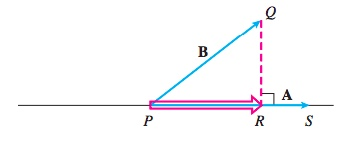
\includegraphics[scale=0.5]{figures_mvc/vector_projection_def}
\end{center}
Physically, if ${\bf b}$ represents a force, then $\text{proj}_{\bf a}{\bf b}$ is the effective force in the ${\bf a}$ direction.

\begin{center}
	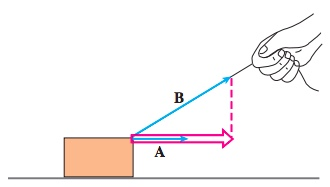
\includegraphics[scale=0.5]{figures_mvc/effective_force_box}
\end{center}	

It is often desirable to express a vector ${\bf b}$ as a sum of two orthogonal vectors. For instance, in mechanics we frequently decompose forces in this way so that we may treat a two-dimensional problem as two one-dimensional problems. We can easily express a vector ${\bf b}$ as such a sum of two vectors, one parallel to some nonzero vector ${\bf a}$ and one orthogonal to ${\bf a}$, in terms of the projection of ${\bf b}$ along ${\bf a}$:
\begin{equation}
\begin{split}
	{\bf b}&={\bf b}_{\parallel}+{\bf b}_{\perp} \\
	&=\text{proj}_{\bf a}{\bf b}+({\bf b}-\text{proj}_{\bf a}{\bf b}).
\end{split}
\end{equation}

\begin{center}
	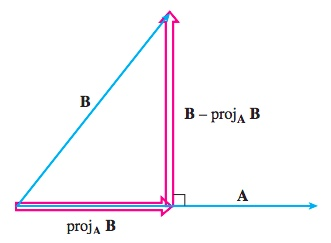
\includegraphics[scale=0.5]{figures_mvc/sum_of_orthogonal_vectors}
\end{center}

\begin{exercise}
	Express ${\bf b}=2{\bf e}_1+{\bf e}_2-3{\bf e}_3$ as the sum of a vector parallel to ${\bf a}=3{\bf e}_1-{\bf e}_2$ and a vector orthogonal to ${\bf a}$.
\end{exercise}

{\color{red} \flushleft {\bf Solution:}
Since ${\bf \hat{a}}\equiv \frac{{\bf a}}{||{\bf a}||}=\frac{3{\bf e}_1-{\bf e}_2}{\sqrt{10}}$, we can write ${\bf b}={\bf b}_{\parallel}+{\bf b}_{\perp}$ with  
\begin{align*}
	{\bf b}_{\parallel}&=({\bf \hat{a}}\cdot {\bf b}){\bf {\hat{a}}}=\frac{1}{2}(3{\bf e}_1-{\bf e}_2)=\frac{1}{2}{\bf a} \\
	{\bf b}_{\perp}&={\bf b}-{\bf b}_{\parallel}=\frac{1}{2}{\bf e}_1+\frac{3}{2}{\bf e}_2-3{\bf e}_3.
\end{align*}}

\subsubsection{The cross product}
There is another vector product which is important in physics, known as the \ti{cross product}. Unlike the dot product, which took two vectors and returned a \ti{scalar}, the cross product takes two vectors and returns another \ti{vector}.

The physical motivation for the cross product is that of \ti{torque}, which is a force that causes a rotation. Suppose we wish to tighten a bolt using a wrench. Applying a force ${\bf F}$ to the handle of the wrench produces a torque which acts along the axis of the bolt to drive the bolt forward. The magnitude of the torque depends on three things:
\begin{enumerate}
	\item The magnitude of ${\bf F}$. That is, how hard we push.
	\item How far out on the handle we apply the force. We denote the vector from the bolt to the point on the handle where the force is applied by ${\bf r}$. This vector is called the \ti{lever arm}. So, the magnitude of the torque also depends on the magnitude of the lever arm.
	\item Finally, the magnitude of the torque depends on the angle with respect to the axis of the handle at which the force is applied. \footnote{The angle we refer to here will be taken to be the \ti{smaller} of the two angles between the force vector and the lever arm.} The torque is zero when this angle is zero (since a force directed \ti{along} the axis of the wrench causes no rotation) and the torque is maximized then the force is perpendicular to the axis of the wrench.
\end{enumerate}
Denoting the torque by $\vec{\tau}$, one observes that 
\begin{equation}\label{eq:magnitude_of_torque}
	||\vec{\tau}||=||{\bf r}||\ ||{\bf F}||\ \sin \theta
\end{equation}
where, again, $\theta$ is the \ti{smaller} of the two angles between ${\bf r}$ and ${\bf F}$.
\begin{center}
	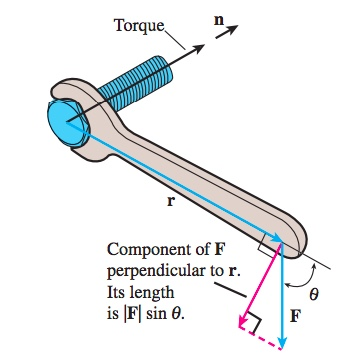
\includegraphics[scale=0.5]{figures_mvc/torque_wrench}
\end{center}
This gives the magnitude of $\vec{\tau}$. Notice that if we take the fingers of our \ti{right} hand and point then along the direction of ${\bf r}$ and then curl them toward ${\bf F}$ through the angle $\theta$ between ${\bf r}$ and ${\bf F}$ (arranged so that their initial points coincide), then our thumb points in the direction of $\vec{\tau}$. This is called the \ti{right-hand rule}. Letting ${\bf n}$ be a unit vector in the direction of $\vec{\tau}$ we have therefore found
\begin{equation}
	\vec{\tau}=||{\bf r}|| \ ||{\bf F}|| \ \sin \theta{\bf n}.
\end{equation}

\begin{example}
The magnitude of the torque exerted by the force ${\bf F}$ about the pivot point $P$ below 

\begin{center}
	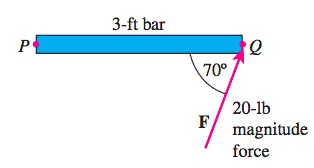
\includegraphics[scale=0.5]{figures_mvc/torque_example}
\end{center}

is 
\begin{align*}
	||\vec{\tau}||=||\overrightarrow{PQ}|| \ ||{\bf F}|| \sin \theta = (3)(20)\sin 70^\circ \approx 56.4 \text{ ft-lb}.
\end{align*}
By the right hand rule, the torque is perpendicular to the plane  containing ${\bf r}$ and ${\bf F}$, and pointing \ti{out} of the page (rather than \ti{into} the page).
\end{example}


\begin{defn}[Cross product]
The \ti{cross product} of two nonzero vectors ${\bf a}$ and ${\bf b}$ is the vector
\begin{equation}
	{\bf a} \times {\bf b}=||{\bf a}|| \ ||{\bf b}|| \ \sin \theta{\bf n}
\end{equation}
where $\theta$ is the angle between ${\bf a}$ and ${\bf b}$ and ${\bf n}$ is a unit vector in the direction determined by the right-hand rule (that is, upon directing the fingers of ones right hand in the direction of ${\bf a}$ and curling them toward ${\bf b}$ through $\theta$, then ones thumb points in the direction of ${\bf n}$ and therefore $\overrightarrow{\tau}$). 

If either ${\bf a}$ or ${\bf b}$ is the zero vector, then we define ${\bf a} \times {\bf b}$ to be ${\bf 0}$.
\end{defn}

If ${\bf a}$ and ${\bf b}$ are both nonzero and if $\theta \neq 0$, then ${\bf a}$ and ${\bf b}$ define a plane, and ${\bf n}$ is perpendicular to this plane. The sense of ${\bf n}$ is the one determined by the right hand rule. 
\begin{center}
	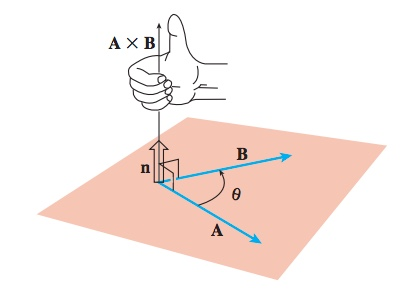
\includegraphics[scale=0.5]{figures_mvc/cross_product}
\end{center}
Thus, 
\begin{center}
	\ti{The cross product ${\bf a} \times {\bf b}$ is a vector perpendicular to both ${\bf a}$ and ${\bf b}$}.
\end{center}

Note that if $\theta=0$ or $\pi$ (that is, if ${\bf a}$ and ${\bf b}$ are parallel, which means they don't determine a plane), then ${\bf a} \times {\bf b}=0$ . Conversely, if ${\bf a}$ and ${\bf b}$ are both non-zero, then we see from the definition that ${\bf a} \times {\bf b}=0$ only if ${\bf a}$ and ${\bf b}$ are parallel. Hence, we have proved the following proposition.

\begin{prop}[Parallel vectors]
	Two nonzero vectors ${\bf a}$ and ${\bf b}$ are parallel if and only if 
	\begin{align*}
		{\bf a} \times {\bf b}=0.
	\end{align*}
\end{prop}

Note that, geometrically, the magnitude of the cross product $||{\bf a} \times {\bf b}||=||{\bf a}|| \ ||{\bf b}||\sin\theta$ is the area of the parallelogram with adjacent sides ${\bf a}$ and ${\bf b}$:
\begin{center}
	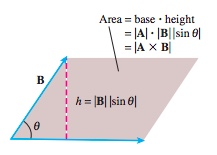
\includegraphics[scale=0.5]{figures_mvc/cross_product_area_of_parallelogram}
\end{center}

Let us now look at the properties of the cross product. Despite its usefulness in physics, it turns out to preserve almost none of the properties of ordinary numerical multiplication. In particular, the cross product is neither commutative nor associative:


\begin{enumerate}[(1)]
	\item ${\bf a} \times {\bf b} \neq {\bf b}  \times {\bf a}$
	\item ${\bf a} \times ({\bf b} \times {\bf c}) \neq ({\bf a} \times {\bf b}) \times {\bf c}$
\end{enumerate}	

Regarding the first of these, if we reverse ${\bf a}$ and ${\bf b}$ in the definition, the only difference is that we rotate ${\bf b}$ into ${\bf a}$ rather than ${\bf a}$ into ${\bf b}$, so the right and rule gives
\begin{equation}
	{\bf a} \times {\bf b}=-{\bf b} \times {\bf a}.
\end{equation}
One the other hand, for the second of these, not only are the magnitudes of ${\bf a} \times ({\bf b} \times {\bf c})$ and $({\bf a} \times {\bf b}) \times {\bf c}$ not necessarily equal, these vectors do not even have to lie in the same plane! \footnote{Applying the definition of each cross product, one finds that ${\bf a} \times ({\bf b} \times {\bf c})$ is parallel to the plane determined by ${\bf b}$ and ${\bf c}$, while $({\bf a} \times {\bf b}) \times {\bf c}$ is parallel to the plane determined by ${\bf a}$ and ${\bf b}$. In particular, there is no reason why the ${\bf a}{\bf b}$-plane and the ${\bf b}{\bf c}$-plane should be the same, since three vectors don't have to lie in the same plane.}

However, vector and scalar distributive laws \ti{do} hold for the cross product:
\begin{prop}[Distributive properties of the cross product]
	\begin{enumerate}[(1)]\hspace{10cm}
	\item $(r{\bf a}) \times (s{\bf b})=(rs)({\bf a} \times {\bf b})$,
	\item ${\bf a} \times ({\bf b} + {\bf c})={\bf a} \times {\bf b}+{\bf a} \times {\bf c}$.
\end{enumerate}
\end{prop}

\begin{pf}
\begin{enumerate}[(1)]\hspace{10cm}
	\item We can verify this formula by applying the definition of the cross product to both sides of the equation:
	\begin{align*}
		||(r{\bf a}) \times (s{\bf b})||&=||(r{\bf a}) || \ ||(s{\bf b})||\sin \theta  \\&=|r| \ |s | \ ||{\bf a} || \ ||{\bf b} || \sin \theta \\
		&=|rs| \ ||{\bf a} || \ ||{\bf b} || \sin \theta \\
		&=||(rs)({\bf a}\times {\bf b})||
	\end{align*}
where we have used the fact that the angle between ${\bf a}$ and ${\bf b}$ is the same as the angle between $r{\bf a}$ and $s{\bf b}$.
	\item To derive this formula, we construct ${\bf a} \times {\bf b}$ in a new way. Draw ${\bf a}$ and ${\bf b}$ from the common point $O$ and construct a plane perpendicular to ${\bf a}$ at $O$.
\begin{center}
	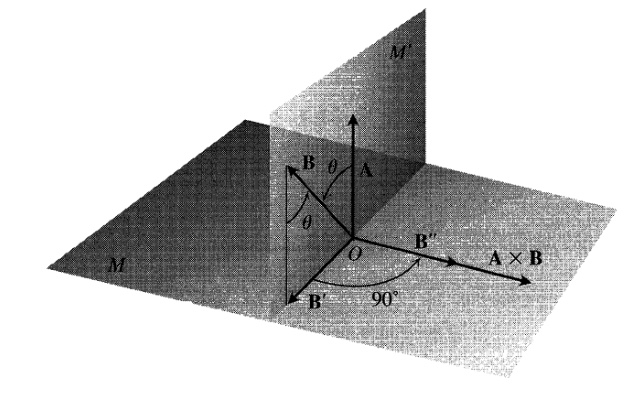
\includegraphics[scale=0.5]{figures_mvc/distributivity_of_the_cross_product_1}
\end{center}
We then project ${\bf b}$ orthogonally onto $M$, yielding a vector ${\bf b}'$ with length $||{\bf b}||\sin \theta$. Finally, we rotate ${\bf b}'$ $90^\circ$ about ${\bf a}$ in the positive sense to produce a vector ${\bf b}''$, and then multiply ${\bf b}''$ by the length of ${\bf a}$. The resulting vector $||{\bf a}||{\bf b}''$ is equal to ${\bf a} \times {\bf b}$ since it has the same direction as ${\bf a} \times {\bf b}$ by construction and 
\begin{align*}
	||{\bf a}|| \ ||{\bf b}''||&=||{\bf a}|| \ ||{\bf b}'|| \ \text{ (since ${\bf b}''$ and ${\bf b}'$ are related by a rotation)} \\
	&=||{\bf a}|| \ ||{\bf b}||\sin\theta \ \text{ (since ${\bf b}'$ is the projection of ${\bf b}$ onto $M$)} \\
	&=||{\bf a} \times {\bf b}||. 
\end{align*}
Now each of these three operations, namely,
\begin{enumerate}
\item projection onto $M$,
\item rotation about ${\bf a}$ through $90^\circ$, 
\item multiplication by the scalar $||{\bf a}||$,
\end{enumerate}
when applied to a triangle whose plane is not parallel to ${\bf a}$, will produce another triangle. \footnote{If the triangle is in a plane parallel to ${\bf a}$ then projection onto $M$ will give a line segment, not a triangle.} If we start with a triangle whose sides are ${\bf b}, {\bf c},$ and ${\bf b}+{\bf c}$ and apply these three steps, we successively obtain
\begin{center}
	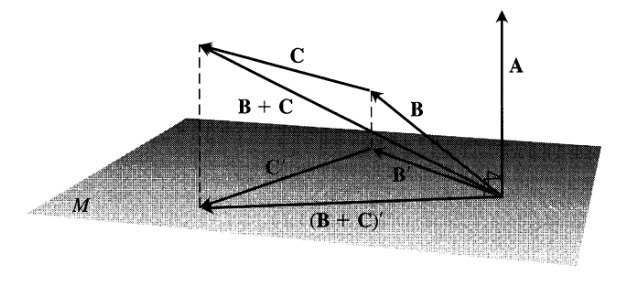
\includegraphics[scale=0.5]{figures_mvc/distributivity_of_the_cross_product_2}
\end{center}
\begin{enumerate}
\item a triangle whose sides are ${\bf b}', {\bf c}',$ and $({\bf b}+{\bf c})'$ satisfying the vector equation
	\begin{align*}
		{\bf b}'+{\bf c}'=({\bf b}+{\bf c})';
	\end{align*}
\item a triangle whose sides are ${\bf b}'', {\bf c}'',$ and $({\bf b}+{\bf c})''$ satisfying the vector equation
	\begin{align*}
		{\bf b}''+{\bf c}''=({\bf b}+{\bf c})'';
	\end{align*}
	and, finally,
\item a triangle whose sides are $||{\bf a}||{\bf b}'',$ $||{\bf a}||{\bf c}''$, and $||{\bf a}({\bf b}+{\bf c})''$ satisfying the vector equation
	\begin{equation}\label{eq:distributive_cross_product}
		||{\bf a}||{\bf b}''+||{\bf a}||{\bf c}''=||{\bf a}||({\bf b}+{\bf c})''.
	\end{equation}
\end{enumerate}
But we have shown above that $||{\bf a}||{\bf b}''={\bf a} \times {\bf b}$, $||{\bf a}||{\bf c}''={\bf a} \times {\bf c}$, and $||{\bf a}||({\bf b}+{\bf c})''={\bf a} \times ({\bf b}+{\bf c})$,
and therefore Eq. \eqref{eq:distributive_cross_product} is equivalent to 
\begin{align*}
	{\bf a} \times {\bf b}+{\bf a} \times {\bf c}={\bf a} \times ({\bf b} + {\bf c}),
\end{align*}
which is the property we wanted to establish.
\end{enumerate}	
\end{pf}

The cross product takes a useful form in  Cartesian coordinates. Let us first work out the various cross products of pairs of the unit vectors ${\bf e}_1, {\bf e}_2, {\bf e}_3$. Applying the definitions of the cross product and the ${\bf e}_i$s, we find 
\begin{align*}
	{\bf e}_i \times {\bf e}_j=\epsilon_{ijk}{\bf e}_k
\end{align*}
for $i,j,k \in \{1,2,3\}$, where
\begin{align*}
	\epsilon_{ijk}=\begin{cases}
		1, \text{ if $(ijk)$ is an even permutation of $(123)$} \\
		-1, \text{ if $(ijk)$ is an odd permutation of $(123)$} \\
		0, \text{ otherwise}
	\end{cases}
\end{align*}
Now let
\begin{align*}
	{\bf a}&=a_1{\bf e}_1+a_2{\bf e}_2+a_3{\bf e}_3 \\
	{\bf b}&=b_1{\bf e}_1+b_2{\bf e}_2+b_3{\bf e}_3 \\
\end{align*} 
We compute ${\bf a} \times {\bf b}$ using the distributive property above and then use the cross products of the ${\bf e}_i$s worked out above to simplify the 9 terms, ending up with \footnote{Those who have previously studied determinants can easily verify that this formula may be written as  
\begin{align*}
	{\bf a} \times {\bf b}=\begin{vmatrix}
		{\bf e}_1 & {\bf e}_2 & {\bf e}_3 \\
		a_1 & a_2 & a_3 \\
		b_1 & b_2 & b_3
	\end{vmatrix},
\end{align*} which is a useful mnemonic to remember the formula in Eq. \eqref{eq:a_cross_b}. We will study determinants in detail in a later unit.}
\begin{equation}\label{eq:a_cross_b}
	{\bf a} \times {\bf b}=(a_2b_3-a_3b_2){\bf e}_1-(a_1b_3-a_3b_1){\bf e}_2+(a_1b_2-a_2b_1){\bf e}_3.
\end{equation}
\fixme{Discuss even odd permutations of $(123)$ and how to remember the signs.}

\begin{exercise}
Compute ${\bf a} \times {\bf b}$ and ${\bf b} \times {\bf a}$ if ${\bf a}=(2,1,1)$ and ${\bf b}=(-4,3,1)$.	
\end{exercise}

{\color{red} \flushleft {\bf Solution:}
\begin{align*}
	{\bf a} \times {\bf b}&=\begin{vmatrix}
		{\bf e}_1 & {\bf e}_2 & {\bf e}_3 \\
		2 & 1 & 1 \\
		-4 & 3 & 1
	\end{vmatrix}
	=(-2,-6,10). \\
	{\bf b} \times {\bf a}&=-{\bf a} \times {\bf b}=(2,6,-10).
\end{align*}
}

\begin{exercise}
Find a vector perpendicular to the plane of $P(1,-1,0), Q(2,1,-1),$ and $R(-1,1,2)$.	
\end{exercise}

{\color{red} \flushleft {\bf Solution:}
Any three lines lie in a plane. We can construct two vectors in this plane:
\begin{align*}
	\overrightarrow{PQ}=(2-1,1-(-1),-1-0)=(1,2-1), \\
	\overrightarrow{PR}=(-1-1,1-(-1),2-0)=(-2,2,2). \\
\end{align*}
A vector perpendicular to this plane is then given by
\begin{align*}
	\overrightarrow{PQ} \times \overrightarrow{PR} =\begin{vmatrix}
		{\bf e}_1 & {\bf e}_2 & {\bf e}_3 \\
		1 & 2 & -1 \\ -2 & 2 & 2
	\end{vmatrix} = (6,0,6).
\end{align*}}

\begin{exercise}
	Find the area of the triangle with vertices $P(1,-1,0), Q(2,1,-1),$ and $R(-1,1,2)$.
\end{exercise}
{\color{red} \flushleft {\bf Solution:}
The area of the parallelogram determined by $P,Q,$ and $R$ is 
\begin{align*}
	||\overrightarrow{PQ} \times \overrightarrow{PR}||=||(6,0,6)||=6\sqrt{2}.
\end{align*}
The triangles area is half of this, or $3\sqrt{2}$.
\begin{center}
	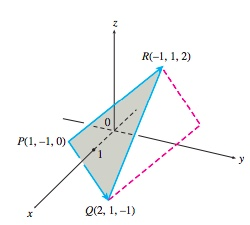
\includegraphics[scale=0.5]{figures_mvc/triangle_area_cross_product}
\end{center}
}

\begin{exercise}
Find a unit vector perpendicular to the plane containing $P(1,-1,0), Q(2,1,-1),$ and $R(-1,1,2)$.	
\end{exercise}

{\color{red} \flushleft {\bf Solution:}
A unit vector perpendicular to the plane is given by
\begin{align*}
	{\bf n}=\frac{\overrightarrow{PQ} \times \overrightarrow{PR}}{||\overrightarrow{PQ} \times \overrightarrow{PR}||}=\frac{(6,0,6)}{6\sqrt{2}}=(1/\sqrt{2},0,1/\sqrt{2}).
\end{align*}}

\subsubsection{The triple scalar product}
Since ${\bf a} \times {\bf b}$ is a vector, note that the product $({\bf a} \times {\bf b}) \cdot {\bf c}$ is defined.

\begin{defn}[Triple scalar product]
	For any vectors ${\bf a}, {\bf b},$ and ${\bf c}$, the \ti{triple scalar product} is defined by
	\begin{align*}
		({\bf a} \times {\bf b}) \cdot {{\bf c}}=||{\bf a} \times {\bf b}|| \ ||{\bf c}|| \cos \theta
	\end{align*}
where $\theta$ is the angle between ${\bf a} \times {\bf b}$ and ${\bf c}$.
\end{defn}

Geometrically, the magnitude of ${\bf a} \times {\bf b} \cdot {{\bf c}}$ is the volume of the parallelepiped whose with adjacent sides ${\bf a}, {\bf b}$, and ${\bf c}$, the number $||{\bf a} \times {\bf b}||$ being the area of the base parallelogram and $||{\bf c}||\cos \theta$ the height of the parallelepiped.
\begin{center}
	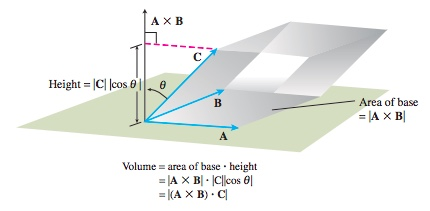
\includegraphics[scale=0.5]{figures_mvc/triple_scalar_product_parallelepiped}
\end{center}
For this reason, the triple scalar product is also called the \ti{box product} of ${\bf a}, {\bf b},$ and ${\bf c}$.

Computing the triple scalar product in Cartesian coordinates, one can verify that 
\begin{equation}\label{eq:triple_scalar_product_formula}
\begin{split}
		({\bf a} \times {\bf b}) \cdot {{\bf c}}&=a_1(b_2c_3-c_3b_2)-a_2(b_1c_3-b_3c_1)+a_3(b_1c_2-c_1b_2)	 \\
		&=\begin{vmatrix}
		a_1 & a_2 & a_3 \\
		b_1 & b_2 & b_3 \\
		c_1 & c_2 & c_3  
	\end{vmatrix}. \\
\end{split}
\end{equation}

\begin{prop}[Cyclic symmetry of triple scalar product]\label{eq:cyclic_symmetry_of_triple_scalar_product}
For any three vectors ${\bf a}, {\bf b},$ and ${\bf c}$, the triple scalar product satisfies
\begin{align*}
	({\bf a} \times {\bf b}) \cdot {\bf c}=({\bf b} \times {\bf c}) \cdot {\bf a}=({\bf c} \times {\bf a}) \cdot {\bf b}.
\end{align*}	
\end{prop}

\begin{pf}
This is straightforward to verify from Eq. \eqref{eq:triple_scalar_product_formula}. For those who know about determinants, the determinant is unchanged under cyclic permutations of the rows.
\end{pf}

\begin{cor}[Interchange of dot and cross product in triple scalar product]
For any three vectors ${\bf a}, {\bf b},$ and ${\bf c}$, the triple scalar product satisfies
\begin{align*}
	({\bf a} \times {\bf b}) \cdot {\bf c}={\bf a}\cdot ({\bf b} \times {\bf c})
\end{align*}	
\end{cor}

\begin{pf}
This follows from Proposition \ref{eq:cyclic_symmetry_of_triple_scalar_product} along with commutativity of the dot product.	
\end{pf}

\begin{exercise}
Find the volume of the parallelepiped with adjacent sides ${\bf a}=(1,2,-1), {\bf b}=(-2,0,3)$, and ${\bf c}=(0,7,-4)$.	
\end{exercise}

{\color{red} \flushleft {\bf Solution:}
This is given by
\begin{align*}
	||{\bf a} \cdot ({\bf b} \times {\bf c})||=\vert \begin{vmatrix}
		1 & 2 & -1 \\ -2 & 0 & 3 \\ 0 & 7 & -4
	\end{vmatrix} \vert = \vert -23 \vert = 23.
\end{align*}}

\subsection{Equations of lines and planes}
\subsubsection{Lines in space}
The coordinate systems of analytic geometry allow us to consider geometric objects such as lines and planes in terms of vectors. These geometric ideas will give us valuable intuition later on in the course when we take a more abstract point of view toward vectors.

First let us recall that any two points define a line. Equivalently, we can also determine a line if we know one point on the line and the slope of the line. 

Let us now work in Cartesian coordinates. Suppose $L$ is a line passing through a point $P_0(x_0,y_0,z_0)$ and parallel to a vector ${\bf v}=v_1{\bf e}_1+v_2{\bf e}_2+v_3{\bf e}_3$. Now let $P(x,y,z)$ be any point in space. In which case will $P(x,y,z)$ to be on the line? This will be the case if the vector $\overrightarrow{P_0P}$ is parallel to ${\bf v}$, that is, if $\overrightarrow{P_0P}$ is a scalar multiple of ${\bf v}$. Therefore,
\begin{defn}[Vector equation for a line]
	The line through $P_0(x_0,y_0,z_0)$ and parallel of ${\bf v}$ is the set of all points $P(x,y,z)$ such that $\overrightarrow{P_0P}=t{\bf v}$, with $-\infty < t < \infty$. This equation is called the \ti{vector equation} of the line.
\end{defn}
In terms of Cartesian coordinates, the vector equation for the line becomes
\begin{align*}
	(x-x_0){\bf e}_1+(y-y_0){\bf e}_2+(z-z_0){\bf e}_3&=t(v_1{\bf e}_1+v_2{\bf e}_2+v_3{\bf e}_3) \\
	&=tv_1{\bf e}_1+tv_2{\bf e}_2+tv_3{\bf e}_3
\end{align*}
which implies
\begin{align*}
	(x-x_0-tv_1){\bf e}_1+(y-y_0-tv_2){\bf e}_2+(z-z_0-tv_3){\bf e}_3={\bf 0}
\end{align*}
and hence
\begin{equation}\label{eq:parametric_equations_line}
	x=x_0+tv_1, \hspace{0.25cm} y=y_0+tv_2, \hspace{0.25cm} z=z_0+tv_3.
\end{equation}
Thus, the vector equation of the line is equivalent to the three scalar equations in Eq. \eqref{eq:parametric_equations_line}, each of which is the usual equation for a line with slope $v_i$ in one variable $t$.

\begin{defn}[Parametric equations for a line]
	The standard parametrization of the line through $P_0(x_0,y_0,z_0)$ and parallel to ${\bf v}=v_1{\bf e}_1+v_2{\bf e}_2+v_3{\bf e}_3$ is given by
	\begin{align*}
		x=x_0+tv_1, \hspace{0.25cm} y=y_0+tv_2, \hspace{0.25cm} z=z_0+tv_3.
	\end{align*}
	These equations are called the (standard) \ti{parametric equations} for the line.
\end{defn}

\begin{exercise}
Find the parametric equations for the line through $(-2,0,4)$ and parallel to ${\bf v}=2{\bf e}_1+4{\bf e}_2-2{\bf e}_3$.	
\end{exercise}

{\color{red} \flushleft {\bf Solution:}
Plugging into Eq. \eqref{eq:parametric_equations_line} gives
\begin{align*}
	x=-2+2t, \hspace{0.25cm} y=4t, \hspace{0.25cm} z=4-2t.
\end{align*}}
\begin{center}
	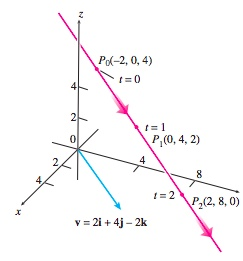
\includegraphics[scale=0.5]{figures_mvc/parametrized_line_example_1}
\end{center}

\begin{example}
	Find parametric equations for the line through $P(-3,2,-3)$ and $Q(1,-1,4)$.
\end{example}

{\color{red} \flushleft {\bf Solution:}
The vector from $P$ to $Q$ is 
\begin{align*}
	\overrightarrow{PQ}&=(1-(-3), -1-2, 4-(-3)) \\
	&=(4,-3,7).
\end{align*}
We take this vector to be our ``${\bf v}$". The point $P_0$ could be either $P$ or $Q$. Arbitrarily choosing it to be $Q$, Eq. \eqref{eq:parametric_equations_line} gives
\begin{align*}
	x=1+4t, \hspace{0.25cm} y=-1-3t, \hspace{0.25cm} z=4+7t.
\end{align*}}

\begin{exercise}
Parametrize the line segment joining the points $P(-3,2,-3)$ and $Q(1,-1,4)$.	
\end{exercise}
{\color{red} \flushleft {\bf Solution:}
We have seen in the previous exercise that the  parametric equations 
\begin{align*}
	x=1+4t, \hspace{0.25cm} y=-1-3t, \hspace{0.25cm} z=4+7t.
\end{align*}
describe an infinite line containing $P$ and $Q$ when we take $-\infty < t < \infty$. To describe the line segment joining $P$ and $Q$, we simply restrict the domain of $t$. We see that the line passes through $P$ at $t=-1$ and $Q=0$. So the line segment joining $P$ and $Q$ is given by 

\begin{align*}
	x=1+4t, \hspace{0.25cm} y=-1-3t, \hspace{0.25cm} z=4+7t.
\end{align*}

with $-1 < t < 0$.}

\subsubsection{Planes in space}
Whereas a line is determined by any two points, a plane is determined by any \ti{three} non-collinear points. Similar to a line, which was equivalently determined by a single point and a slope, a plane can also be determined by a single point and a ``slope". The direction of the plane is determined by a normal vector ${\bf n}=n_1{\bf e}_1+n_2{\bf e}_2+n_3{\bf e}_3$. 

Let us now repeat the question we asked before: given a point $P_0(x_0,y_0,z_0)$ on the plane and a vector ${\bf n}$ normal to the plane, what is the condition for an arbitrary point in space $P(x,y,z)$ to lie on the plane? If $P$ lies in the plane, the $\overrightarrow{P_0P}$ is a vector lying in the plane. Then, since ${\bf n}$ is normal to the plane, we must have that ${\bf n} \cdot \overrightarrow{P_0P}=0$.

\begin{center}
	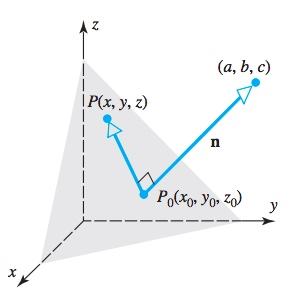
\includegraphics[scale=0.5]{figures_mvc/vector_equation_of_a_plane}
\end{center}

\begin{defn}[Vector equation for a plane]
	The \ti{vector equation} of the plane through $P_0(x_0,y_0,z_0)$ and normal to ${\bf n}=n_1{\bf e}_1+n_2{\bf e}_2+n_3{\bf e}_3$ is given by
	\begin{equation}
		{\bf n} \cdot \overrightarrow{P_0P}=0.
	\end{equation}
\end{defn}

As before, we can expand this equation in Cartesian coordinates to obtain

\begin{defn}[The component equation of a plane]
	The component equation of a plane through $P_0(x_0,y_0,z_0)$ and normal to ${\bf n}=n_1{\bf e}_1+n_2{\bf e}_2+n_3{\bf e}_3$ is given by
	\begin{equation}
		n_1(x-x_0)+n_2(y-y_0)+n_3(z-z_0)=0.
	\end{equation}
	This can be simplified to 
	\begin{equation}
		n_1x+n_2y+n_3z=c
	\end{equation}
	where $c=n_1x_0+n_2y_0+n_3z_0$.
\end{defn}

\begin{exercise}
Find an equation for the plane through $P_0(-3,0,7)$ perpendicular to ${\bf n}=(5,2,-1)$.	
\end{exercise}

{\color{red} \flushleft {\bf Solution:}
The component equation is 
\begin{align*}
	5(x-(-3))+2(y-0)+(-1)(z-7)=0,
\end{align*}
Simplifying, we obtain
\begin{align*}
	5x+15+2y-z+7&=0 \\
	5x+2y-z&=-22.
\end{align*}}

\begin{exercise}
Find the point where the line 
\begin{align*}
	x=\frac{8}{3}+2t, \hspace{0.25cm} y=2t, \hspace{0.25cm} z=1+t
\end{align*}	
intersects the plane $3x+2y+6z=6$.
\end{exercise}

{\color{red} \flushleft {\bf Solution:}
The point $(\frac{8}{3}+2t, 2t, 1+t)$ lies in the plane if its coordinates satisfy the equation of the plane; that is, if
\begin{align*}
	3(\frac{8}{3}+2t)+2(-2t)+6(1+t)=6
\end{align*}
This has a solution at $t=-1$, so the point of intersection is 
\begin{align*}
	(x,y,z)\vert_{t=-1}=(\frac{2}{3},2,0).
\end{align*}}

\begin{exercise}
\begin{enumerate}[(a)]
	\item Find a vector parallel to the line of intersection of the planes $3x-6y-2z=15$ and $2x+y-2z=5$.	
	\item Find parametric equations for the line in which these planes intersect.
\end{enumerate}
\end{exercise}

\subsection{$n$-dimensional space}
As we just have seen, the geometry of three-dimensional space is more complicated and harder to visualize than the geometry of one- or two-dimensional space. However, we have also seen that if we work in Cartesian coordinates, there is a remarkably simple structural resemblance between vectors in each of these spaces.

Consider a vector in each of these spaces:
\begin{enumerate}[(1)]
	\item If ${\bf v}=v_1{\bf e}_1$, then
		\begin{align*}
			||{\bf v}||=\sqrt{(v_1)^2}=|v_1|.
		\end{align*}
	\item If ${\bf v}=v_1{\bf e}_1+v_2{\bf e}_2$, then
		\begin{align*}
			||{\bf v}||=\sqrt{(v_1)^2+(v_2)^2.}
		\end{align*}
	\item If ${\bf v}=v_1{\bf e}_1+v_2{\bf e}_2+v_3{\bf e}_3$, then
		\begin{align*}
			||{\bf v}||=\sqrt{(v_1)^2+(v_2)^2+(v_3)^2}.
		\end{align*}
\end{enumerate} 
Similarly, in each dimension, we have seen that the basic operations of vector addition and scalar multiplication are given by

\begin{enumerate}[(1)]
	\item If ${\bf v}=v_1{\bf e}_1,{\bf w}=w_1{\bf e}_1,$ and $k$ a scalar, then
	\begin{align*}
		{\bf v}+{\bf w}&=(v_1+w_1){\bf e_1} \\
		k{\bf v}&=(kv_1){\bf e}_1.
	\end{align*}
	\item If ${\bf v}=v_1{\bf e}_1+v_2{\bf e}_2,{\bf w}=w_1{\bf e}_1+w_2{\bf e}_2,$ and $k$ a scalar, then
	\begin{align*}
		{\bf v}+{\bf w}&=(v_1+w_1){\bf e}_1+(v_2+w_2){\bf e}_2 \\
		k{\bf v}&=(kv_1){\bf e}_1+(kv_2){\bf e}_2.
	\end{align*}
	\item If ${\bf v}=v_1{\bf e}_1+v_2{\bf e}_2+v_3{\bf e}_3,{\bf w}=w_1{\bf e}_1+w_2{\bf e}_2+w_3{\bf e}_3,$ and $k$ a scalar, then
	\begin{align*}
		{\bf v}+{\bf w}&=(v_1+w_1){\bf e}_1+(v_2+w_2){\bf e}_2+(v_3+w_3){\bf e}_3 \\
		k{\bf v}&=(kv_1){\bf e}_1+(kv_2){\bf e}_2+(kv_3){\bf e}_3.
	\end{align*}
\end{enumerate}

We see that, once our rules and definitions are set, we don't have to worry about how difficult the geometry is. Except for the fact that we have an extra component to work with, there is no structural difference between working with vectors in two-dimensional space or three-dimensional space.

In fact, this construction has a natural generalization.

\begin{defn}[$n$-dimensional space]
	Consider the set of all $n$-tuples of real numbers $(x_1,x_2,\cdots,x_n)$. We denote this set by $\mathbb{R}^n$.
\end{defn}

\begin{example}
	The sets of all one-, two-, and three-tuples of real numbers, which we have been considering so far, are denoted $\mathbb{R}, \mathbb{R}^2,$ and $\mathbb{R}^3$, respectively.
\end{example}

Through the coordinate correspondence, $\mathbb{R}^n$ is geometrically obtained by introducing Cartesian coordinates for an $n$-dimensional Euclidean space. While the geometry of such a space is impossible to draw, we can define vectors in $\mathbb{R}^n$ by generalizing the definitions in $\mathbb{R}^3$:
\begin{itemize}
	\item A vector with its initial point at the origin $(0,0,\cdots,0)$ and terminal point at $(v_1,v_2,\cdots,v_n)$ will have components $(v_1,v_2,\cdots,v_n)$. Two vectors ${\bf v}$ and ${\bf w}$ are equal if 
	\begin{align*}
		v_1=w_1, \hspace{0.25cm} v_2=w_2, \hspace{0.25cm} \cdots \hspace{0.25cm} v_n=w_n
	\end{align*}
	The zero vector has components ${\bf 0}=(0,0,\cdots,0)$.
	\item We define vector addition and scalar multiplication as before: introducing unit vectors ${\bf e}_1, {\bf e}_2, \cdots, {\bf e}_2$ pointing along the coordinate axes, for two vectors ${\bf v}$ and ${\bf w}$ in $n$-dimensional space and $k$ any scalar,
\begin{align*}
	(v_1{\bf e}_1+\cdots+v_n{\bf e}_n)+(w_1{\bf e}_1+\cdots+w_n{\bf e}_n)&=(v_1+w_1){\bf e}_1+\cdots +(v_n+w_n){\bf e}_n \\
	k(v_1{\bf e}_1+\cdots+v_n{\bf e}_n)&=(kv_1){\bf e}_1+\cdots+(kv_n){\bf e}_n.
\end{align*}
\item The dot product of two vectors ${\bf v}$ and ${\bf w}$ in $\mathbb{R}^n$ is given by
\begin{align*}
	{\bf v}\cdot {\bf w}=v_1w_1+\cdots v_nw_n.
\end{align*}
\item The cross product is special to $\mathbb{R}^3$. There is no analog of the cross product for $\mathbb{R}^n$, when $n>3$. \footnote{It is possible to define a product which takes as input $n-1$ $n$-dimensional vectors and produces a vector perpendicular to each one of these, but we will not use such an operation in this course.}
\end{itemize}

We can use these definitions to show that the structural properties of vectors in $\mathbb{R}^3$ continue to hold for vectors in $\mathbb{R}^n$.

\begin{thm}[Properties of vectors in $\mathbb{R}^n$]
If ${\bf u}, {\bf v},$ and ${\bf w}$ are vectors in $\mathbb{R}^n$, and if $k$ and $m$ are scalars, then:
	\begin{enumerate}[(a)]
		\item ${\bf u}+{\bf v}={\bf v}+{\bf u}$
		\item $({\bf u}+{\bf v})+{\bf w}={\bf u}+({\bf v}+{\bf w})$
		\item ${\bf u}+{\bf 0}={\bf 0}+{\bf u}={\bf u}$
		\item ${\bf u}+(-{\bf u})={\bf 0}$
		\item $k({\bf u}+{\bf v})=k{\bf u}+k{\bf v}$
		\item $(k+m){\bf u}=k{\bf u}+m{\bf u}$
		\item $k(m{\bf u})=(km){\bf u}$
		\item $1{\bf u}={\bf u}$
		\item $0{\bf v}={\bf 0}$
		\item $k{\bf 0}={\bf 0}$
		\item $(-1){\bf v}=-{\bf v}$
	\end{enumerate}
\end{thm}

\begin{pf}
Exercise.	
\end{pf}

This theorem allows us to compute in $\mathbb{R}^n$ without explicitly writing out all the components, which can be extremely cumbersome. For instance, the previous theorem can be used to prove that if ${\bf x}+{\bf a}={\bf b}$, then ${\bf x}={\bf b}-{\bf a}$:
\begin{align*}
	{\bf x}+{\bf a}&={\bf b} \\
	({\bf x}+{\bf a})+(-{\bf a})&={\bf b}+(-{\bf a}) \\
	{\bf x}+({\bf a}+(-{\bf a}))&={\bf b}-{\bf a} \\
	{\bf x}+{\bf 0}&={\bf b}-{\bf a} \\
	{\bf x}&={\bf b}-{\bf a}.
\end{align*}

Finally, it is common for addition, subtraction, and scalar multiplication to be used in combination to form new vectors. For example, if ${\bf v}_1, {\bf v}_2,$ and ${\bf v}_3$ are vectors in $\mathbb{R}^n$, then in this way we can form the vectors
\begin{align*}
	{\bf u}=2{\bf v}_1+3{\bf v}_2+{\bf v}_3 \text{ and } {\bf w}=7{\bf v}_1-6{\bf v}_2+8{\bf v}_3.
\end{align*}
This motivates the following definition.

\begin{defn}[Linear combination]
	If ${\bf w}$ is a vector in $\mathbb{R}^n$, then ${\bf w}$ is said to be a \ti{linear combination} of the vectors ${\bf v}_1, {\bf v}_2, \cdots, {\bf v}_r$ in $\mathbb{R}^n$ if it can be expressed in the form
	\begin{align*}
		{\bf w}=k_1{\bf v}_1+k_2{\bf v}_2+\cdots +k_r{\bf v}_r
	\end{align*}
	where $k_1,k_2,\cdots,k_r$ are scalars. The scalars are called the \ti{coefficients} of the linear combination.
	
	In the case where $r=1$, this becomes ${\bf w}=k_1{\bf v}_1$, so a linear combination of a single vector is just a scalar multiple of that vector.
\end{defn}

\subsubsection{Applications of $n$-dimensional space}
\fixme{Finish.}
\end{document}

